%\documentclass[12pt]{report}
\documentclass[12pt]{article}
\usepackage[english]{babel}
\usepackage{natbib}
\usepackage{url}
\usepackage[utf8x]{inputenc}
\usepackage{amsmath}
\usepackage{algorithmic}
\usepackage{graphicx}
\graphicspath{{images/}}
\usepackage{parskip}
\usepackage{pgf,tikz,pgfplots}
\pgfplotsset{compat=1.15}
\usepackage{mathrsfs}
\usetikzlibrary{arrows}
\usepackage{fancyhdr}
\usepackage{vmargin}
\usepackage{algorithm2e}
\usepackage{amsmath}
\usepackage{float}

%------------- For bib ------------------
%\usepackage[utf8]{inputenc}
%\usepackage[english]{babel}
%\usepackage{biblatex}
%\addbibresource{sample.bib}
\usepackage{natbib}
\bibliographystyle{abbrvnat}
\setcitestyle{authoryear,open={((},close={))}}
%------------- For bib ------------------

%\renewcommand{\thesection}{\arabic{section}
\setmarginsrb{3 cm}{2.5 cm}{3 cm}{2.5 cm}{1 cm}{1.5 cm}{1 cm}{1.5 cm}
\newcommand{\ackname}{Acknowledgements}

%\title{A Project on \vspace{0.5cm}\\
\title{Project Report on \vspace{0.5cm}\\
\emph{ISP Censorship Analyzer}	}							
\author{Mahim Mahbub\\
Md Hasan Al Kayem\\
Md. Imran Hasan}								
\date{\today}											

\makeatletter
\let\thetitle\@title
\let\theauthor\@author
\let\thedate\@date
\makeatother

\pagestyle{fancy}
\fancyhf{}
%\rhead{\theauthor}
\lhead{ISP Censorship Analyzer}
\cfoot{\thepage}
\begin{document}

%%%%%%%%%%%%%%%%%%%%%%%%%%%%%%%%%%%%%%%%%%%%%%%%%%%%%%%%%%%%%%%%%%%%%%%%%%%%%%%%%%%%%%%%%

\begin{titlepage}
	\centering
    \vspace*{0.5 cm}
    
\includegraphics[height=2.5cm]{logo1.png}\\[1.0 cm]	% University Logo
    \textsc{\large Bangladesh University of Engineering and Technology}\\[2.0 cm]	% University Name
	\rule{\linewidth}{0.2 mm} \\[0.4 cm]
	{ \huge \bfseries \thetitle}\\
	\rule{\linewidth}{0.2 mm} \\[1.5 cm]
	\textsc{\Large Course Code: CSE 326}\\[0.5 cm]				% Course Code
	\textsc{\large Course Name: Information System Design Sessional}\\[0.5 cm]				% Course Name
    \vspace{1cm}
	\begin{minipage}{0.4\textwidth}
		\begin{flushleft} \large
			\emph{Author:}\\
			\theauthor
			\end{flushleft}
			\end{minipage}~
			\begin{minipage}{0.4\textwidth}
			\begin{flushright} \large
			\emph{Student ID:} \\
			1505022\\
			1505023\\
			1505026
		\end{flushright}
	\end{minipage}\\[2 cm]
	
	{\large \thedate}\\[2 cm]
 
	\vfill
	
\end{titlepage}

%%%%%%%%%%%%%%%%%%%%%%%%%%%%%%%%%%%%%%%%%%%%%%%%%%%%%%%%%%%%%%%%%%%%%%%%%%%%%%%%%%%%%%%%%

\newpage
\subsection*{\ackname}
%We would like to thank
We would like to express our gratitude and appreciation to our respected teachers
\begin{itemize}
\item Dr. Anindya Iqbal Sir\\Associate Professor\\Department of CSE, BUET
\item Mahjabin Nahar Madam\\Lecturer\\Department of CSE, BUET
\item Nafis Irtiza Tripto Sir\\Lecturer\\Department of CSE, BUET
\end{itemize}


\newpage
\tableofcontents
\newpage
\listoffigures
\newpage

%%%%%%%%%%%%%%%%%%%%%%%%%%%%%%%%%%%%%%%%%%%%%%%%%%%%%%%%%%%%%%%%%%%%%%%%%%%%%%%%%%%%%%%%%
\section{Introduction}
People all over the world has different opinion regarding censorship in any communication medium. Internet being the most popular communication medium of this age, has 
enhanced this dispute. At one end of the spectrum, countries like China and Russia censor almost all internet traffic. On the other end, nations like United states and Japan have traditionally been observed as supporters of internet freedom. In between, countries like Bangladesh are attempting to apply internet censorship over the last few years. According to Freedom on the Net, Bangladesh is among the list of countries that have partly free internet. However, the project failed to identify the mechanisms of internet censorship in Bangladesh. Therefore, we aim to investigate the existing internet censorship mechanism in Bangladesh.


Internet censorship in any country is generally controlled by the country’s government while the country’s public and private internet service providers implement the censorship. First step of our project will be the collection of blocked websites from Bangladesh government. With required permissions, Various governmental organizations like Access to Information, Bangladesh Telecommunication Regulatory Commission, and Ministry of Information Technology can help us collect this information.


The next step of our project will be to investigate whether all the major internet service providers enforce the government provided censorship in their traffic. In that regard, one could use existing tools like open observatory of network interference (OONI), BlockCheck, and cachebrowser but these tools are subjected to high percentage of false positives and false negatives. Therefore, we will build an automated system from bottom up to verify results ourselves. This will be a desktop application and could be used by anyone.
%\newpage
For major internet service providers, we will be testing with mobile networks such as Banglalink, Grameenphone, Robi, etc and try to understand the behaviour of these mobile networks with respect to censored websites. Using our system, we will try to understand how major internet service providers enforce the censorship. Different techniques to enforce the censorship include DNS blocking, TCP/IP packet filtering, HTTP filtering, Active probing, etc. Among these techniques, the effort to implement and elude the censorship varies widely. Moreover, these techniques have other side effects like unexpected traffic blocking and sudden internet throttling and shutdown. Therefore, it is of much importance to study the approaches adopted by major internet service providers.


\section{System overview}
%Brief description of the major sub-systems, actors of your system. 
Our system has 6 major subsystems. Brief descriptions of these major subsystems are listed below.
\begin{enumerate}
    \item \textbf{Authentication Subsystem} : This subsystem simply makes a user login to his/her account and if account does not exist, then he/she can register and make an account using email address. A simple email verification also exists.
    \item \textbf{DNS Blocking Check Subsystem}: This subsystem, in short, checks whether a given url is censored with respect to DNS blocking censorship technique.
    \item \textbf{HTTP Filtering Check}: This subsystem, in short, checks whether a given url is censored with respect to HTTP filtering censorship technique.
    \item \textbf{TCP Filtering Check}: This subsystem, in short, checks whether a given url is censored with respect to TCP filtering censorship technique.
    \item \textbf{Censorship Tracking}: This subsystem, in short, checks whether a given url is censored and finds out which method is used. Above subsystems work as kind of independent checking whereas this is kind of a sequential checking starting with DNS checking, then TCP filtering checking and finally ending with HTTP filtering checking.
    \item \textbf{General Facility}: This subsystem is for the interaction with the user. Users can check status using ping, tracert etc. Users can also review their history.
\end{enumerate}
%\newpage
The actors of our system include: 
\begin{itemize}
    \item \textbf{Logged User}: This is a primary business actor. A user must first have to be registered and logged in to have access to the system.
    \item \textbf{Admin}: This is a primary system actor. Admin has the right to delete or modify any data stored in the database of system server.
    \item \textbf{System Server}: External Server Actor. Stores data of the user and the reports generated.
    \item \textbf{Local Server (ISP)}: Another External Server Actor. Responds to dns query request. Either sends an IP (or a list of IPs) or does not send back anything.
    \item \textbf{Proxy Server (eg. TOR Browser)}: Another External Server Actor. Responds to dns query request. Sends an IP (or a list of IPs) or does not send anything if a url is invalid.
    \item \textbf{Web Server}: Another External Server Actor. System tries to initiate a TCP 3-way handshake. %Also tries to retrieve data from web server, depending on which use case is executing.
\end{itemize}

\section{Use case diagram}

%----------------- Use case Authentication  --------------------------------------

\subsection{Authentication Subsystem}
\begin{figure}[h]
    \centering
    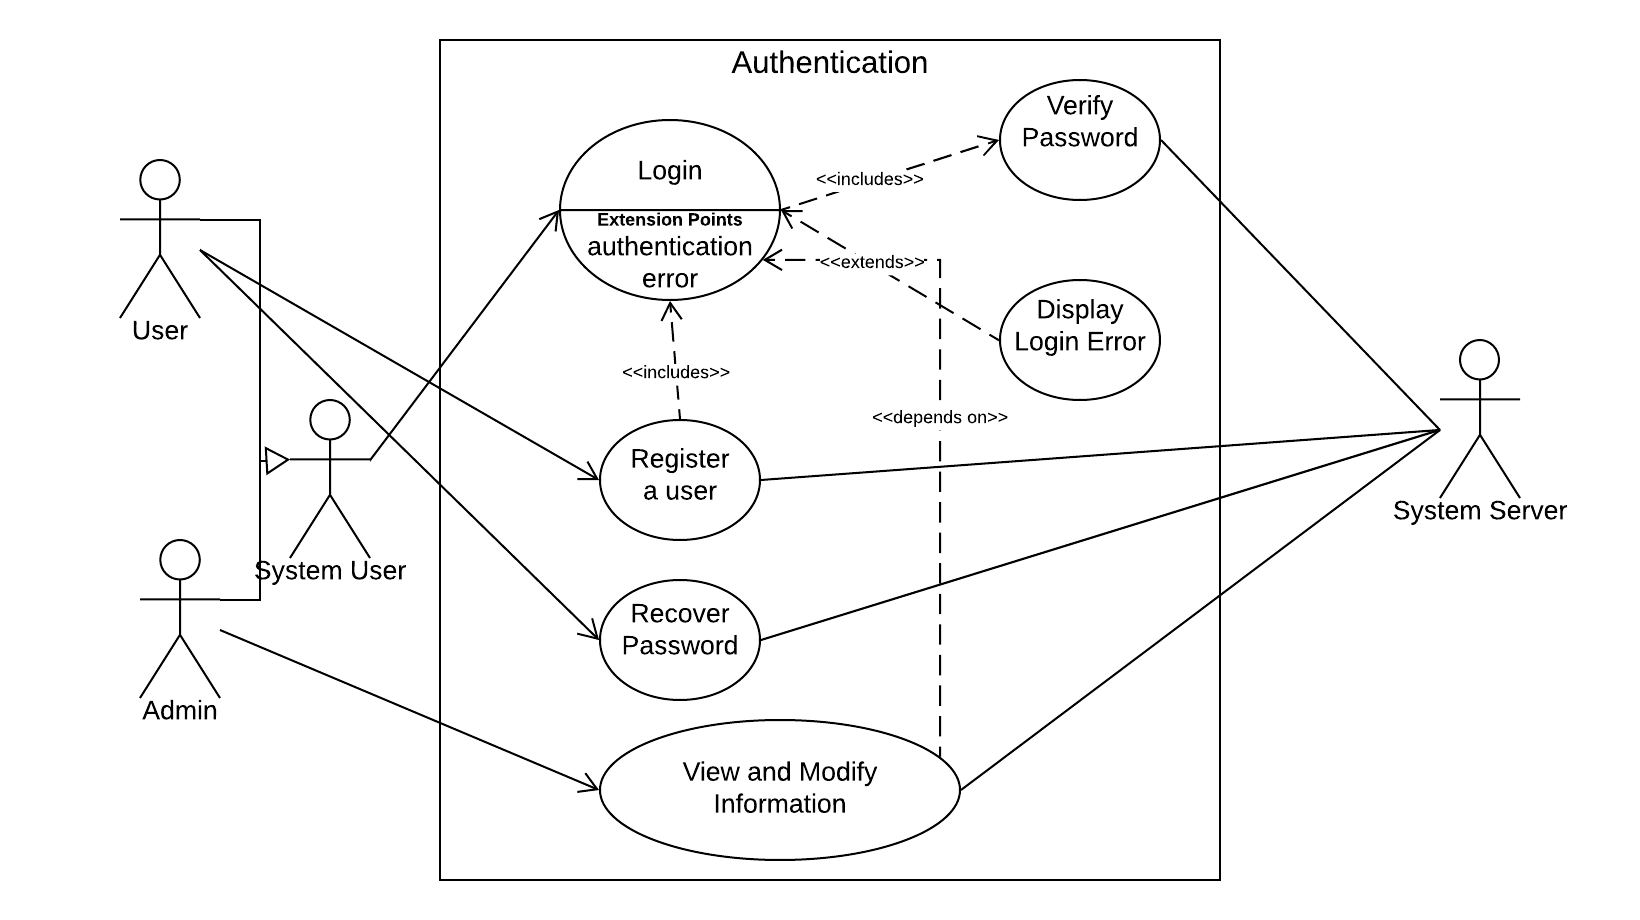
\includegraphics[width=\textwidth]{uclin.png}
    \caption{Use Case of Authentication Subsystem}
    \label{fig:uclin}
\end{figure}

In authentication subsystem, a user can register in this system and log in to use full feature of our system. Admin can view and modify information of whole system server.

%----------------- Use case DNS Blocking ----------------------------------
\newpage
\subsection{DNS Blocking Check}
\begin{figure}[h]
    \centering
    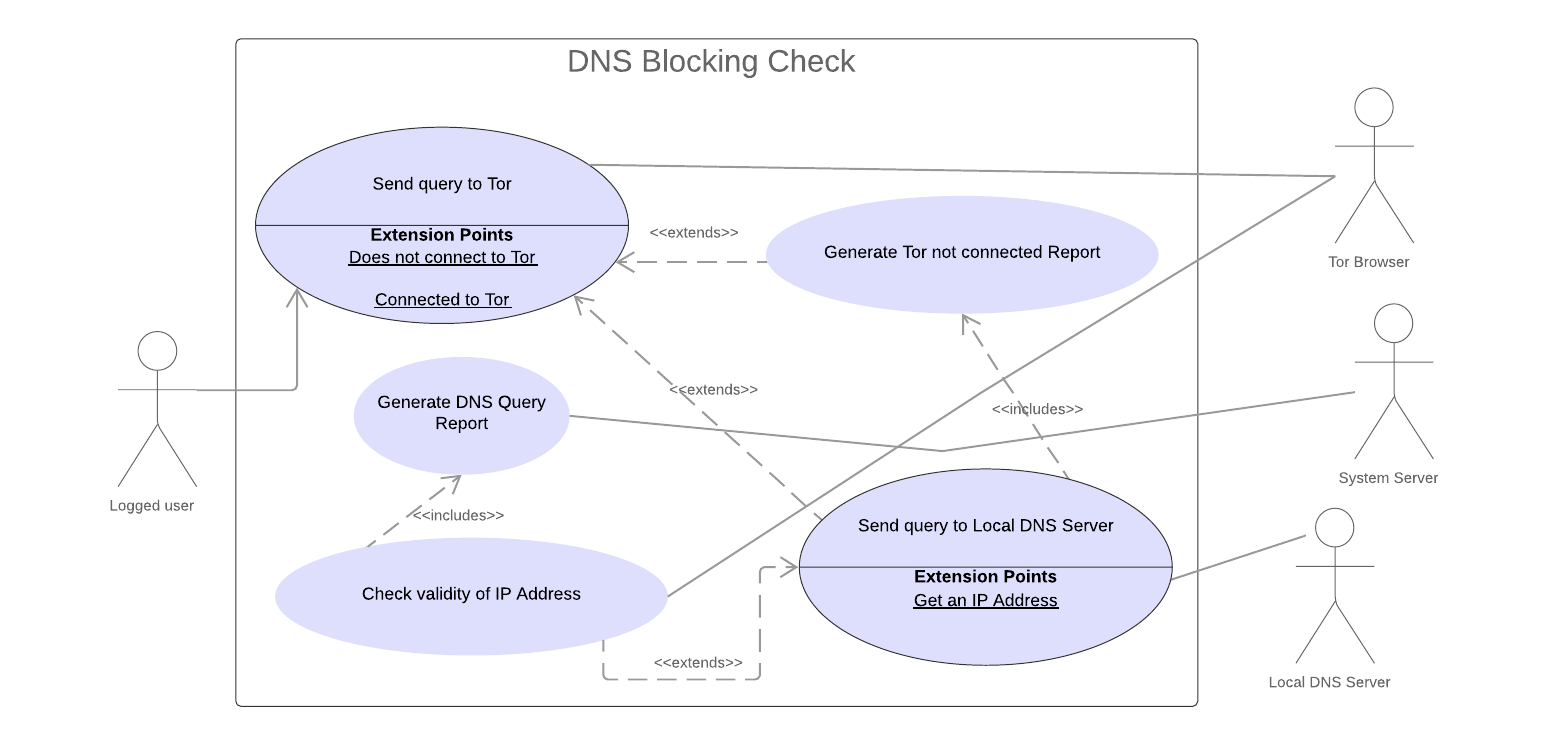
\includegraphics[width=\textwidth]{ucdns.png}
    \caption{Use Case of DNS Blocking Check Subsystem}
    \label{fig:ucdns}
\end{figure}
For DNS Blocking Check subsystem, We will try to figure out if a given url is blocked using DNS Blocking or DNS poisoning techniques. First to verify the validity of url, we will send a query to Tor Browser (used for proxy server). If it does not connect then the url is invalid and we will generate invalid url report (Does not connect to Tor report). If it does connect, from Tor browser, we shall retrieve IP(s) against this url and do the same query (nslookup) with the local server (ISP). If we do not get any IP address, then we can conclude that DNS related censorship was used. Otherwise, using Tor again, we shall check the validity of the IP(s) got from Local Server(ISP) and generate the report accordingly.

%----------------- Use case HTTP Filtering ----------------------------------
\newpage
\subsection{HTTP Filtering Check}

\begin{figure}[h]
    \centering
    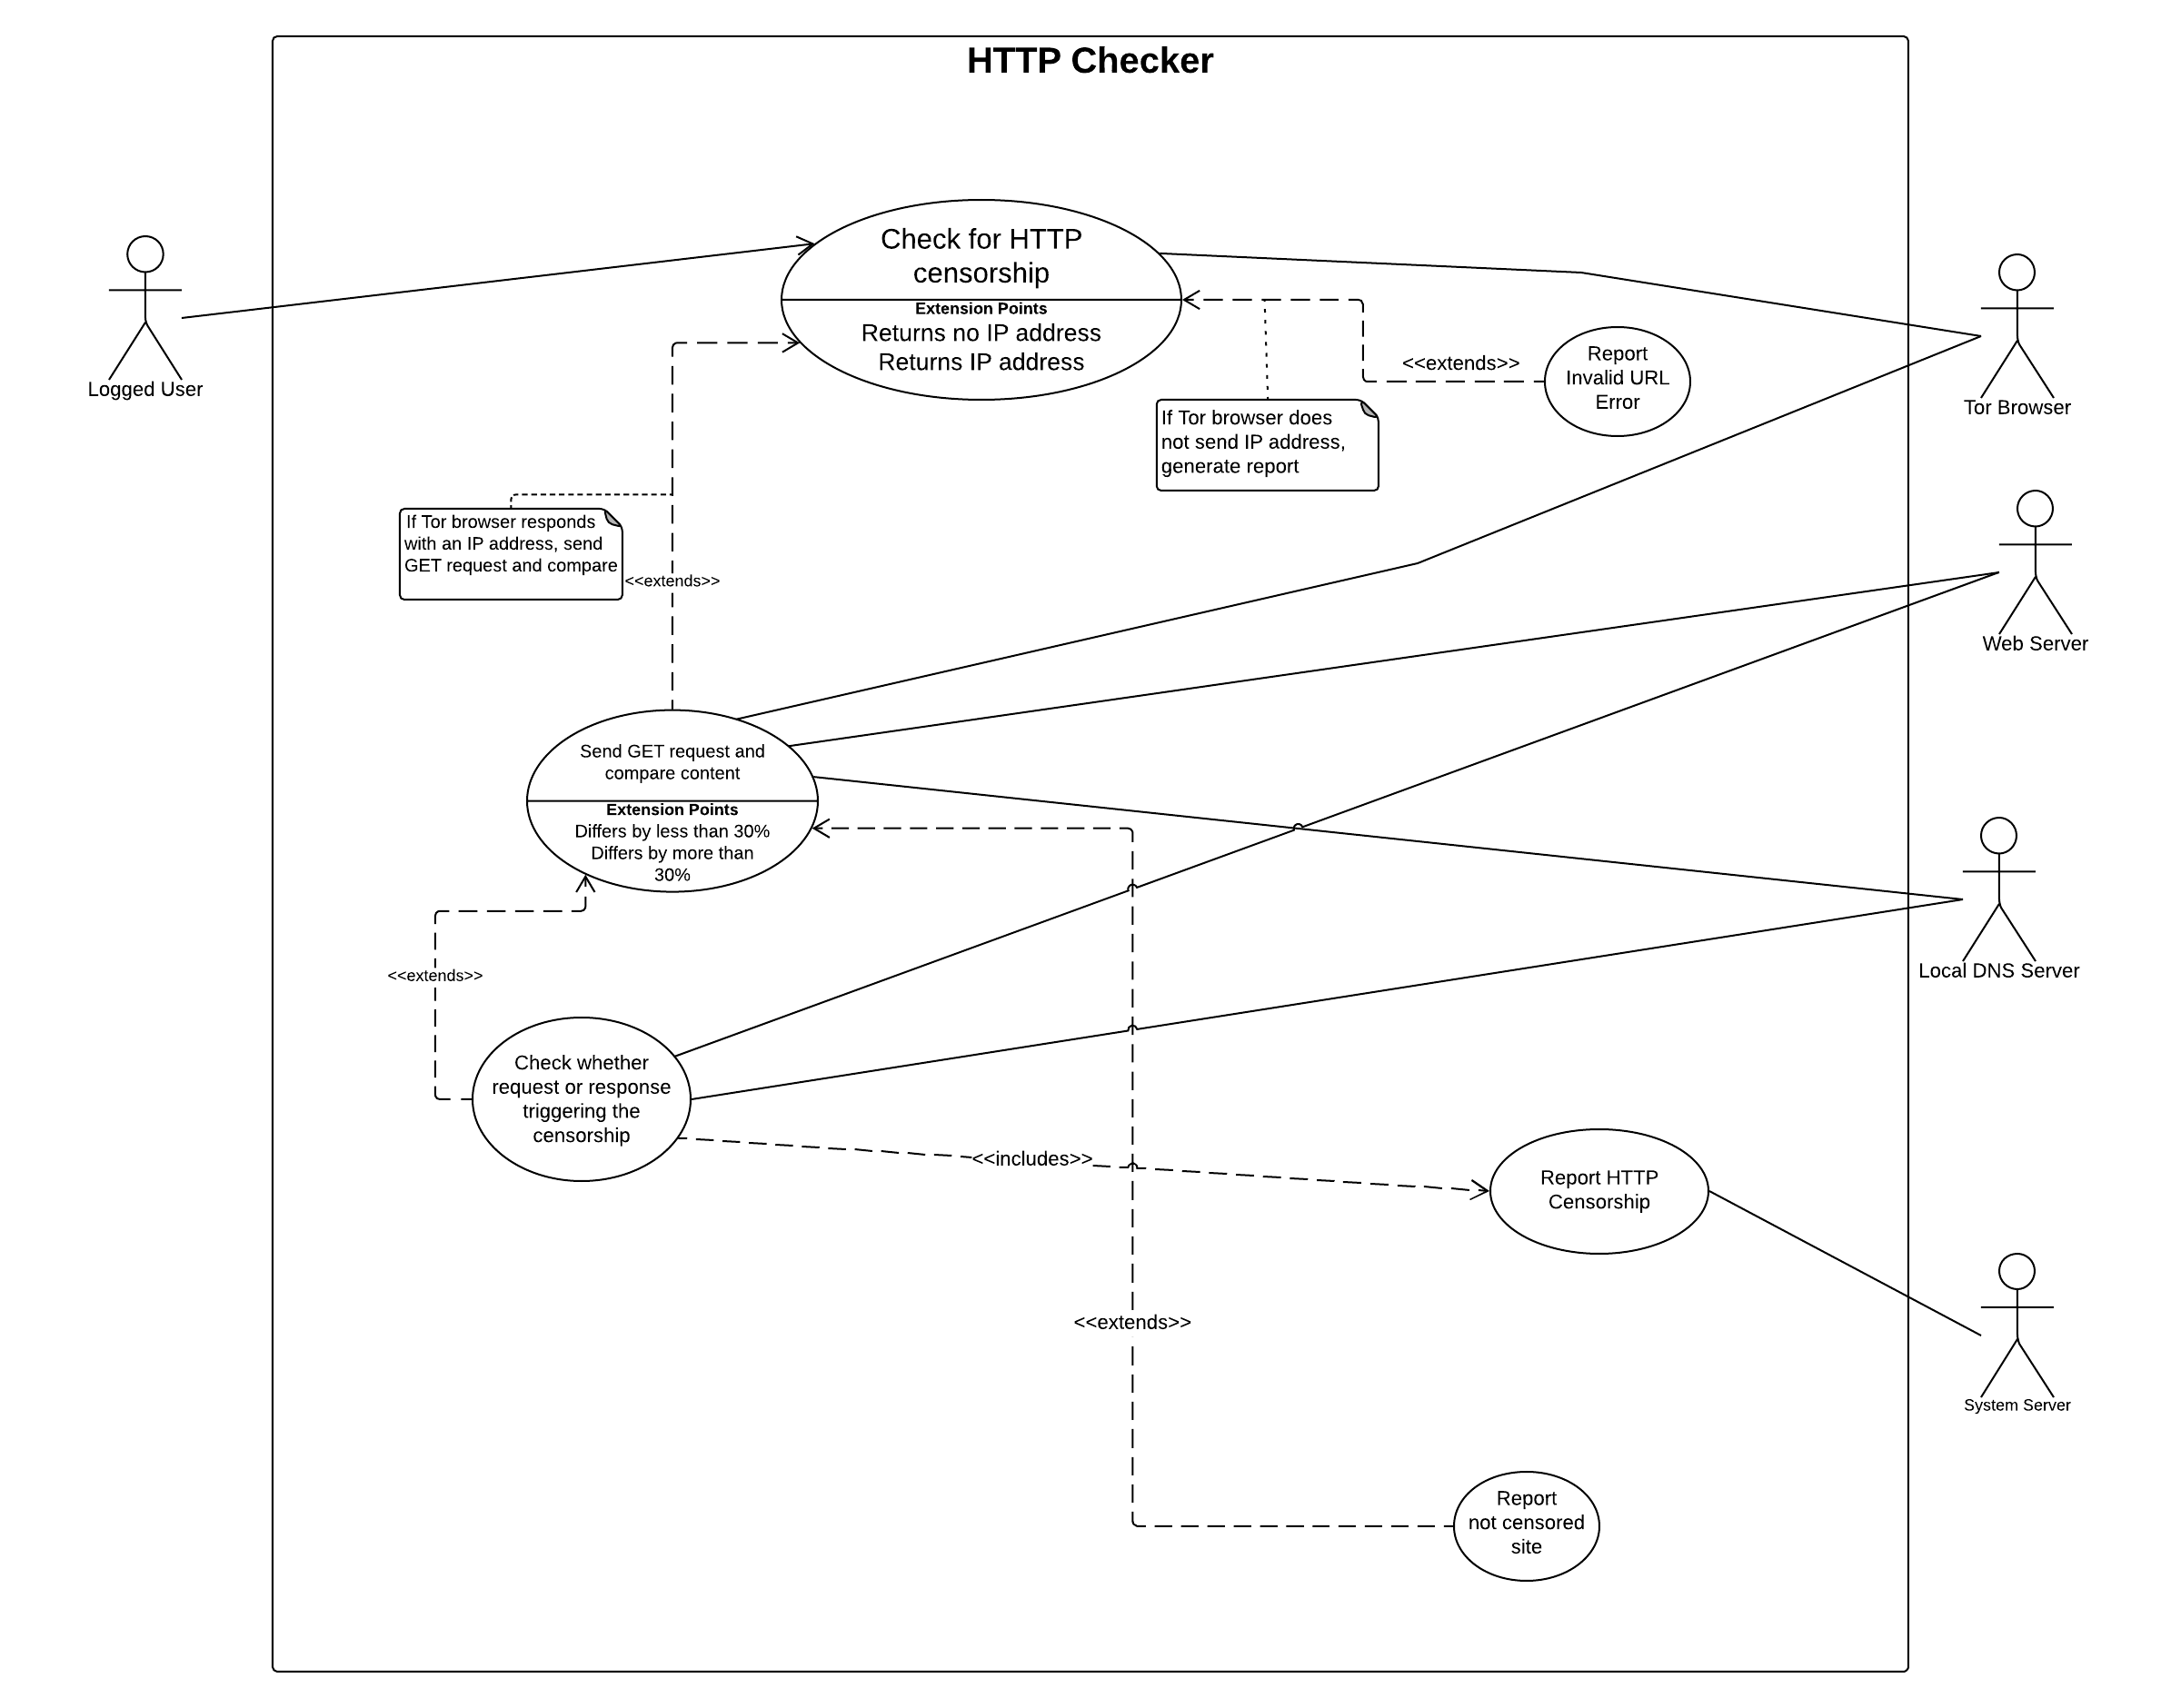
\includegraphics[width=\textwidth]{uchttp.png}
    \caption{Use Case of HTTP Filtering Check Subsystem}
    \label{fig:uchttp}
\end{figure}
For HTTP Filtering, we will assume that our local server does return IP(s) for a given url successfully (i.e. no DNS related censorship for this url). 
So, after initial validation of url (i.e. checking if proxy browser eg. TOR browser does connect to the url), we shall use this IP(or list of IPs) to send HTTP GET request(s) and retrieve the content from proxy browser. Then by doing nslookup using local server, we shall send the same GET request(s) using IP(s) obtained from local server to retrieve this content. We shall then compare the two contents and if their mismatch lies beyond a certain threshold (which shall be experimentally determined), we would conclude HTTP related censorship and form a report accordingly for users to analyze.

%----------------- Use case TCP Filtering ----------------------------------
\newpage
\subsection{TCP Filtering Check}

\begin{figure}[h]
    \centering
    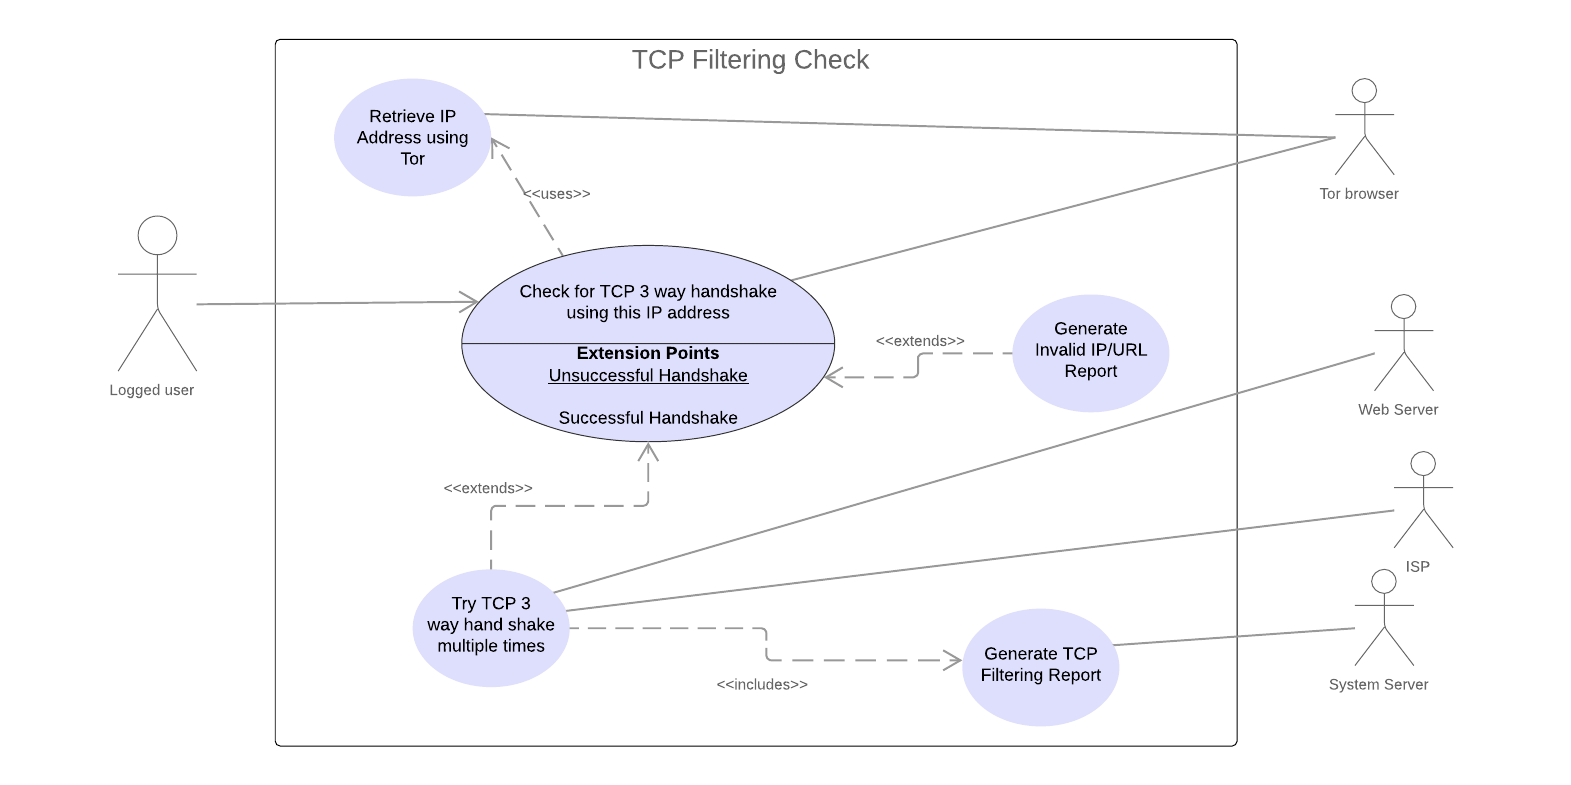
\includegraphics[width=\textwidth]{uctcp.png}
    \caption{Use Case of TCP Filtering Check Subsystem}
    \label{fig:uctcp}
\end{figure}

For TCP filtering as well, we shall assume no DNS related censorship has occured (since our three methods could be checked independently and in conjunction as well). With this assumption, we shall retrieve IP address(or list of IPs) from a proxy browser(eg. TOR) and try to establish a TCP three-way handshake with the proxy server. This is done to ensure that the website is not temporarily down or has not been moved temporarily when we are running our system. Then by getting IP(s) from local server, we shall try to establish three-way handshake multiple times with the website after regular intervals. If all of the attempts are unsuccessful, we would conclude that there may be TCP filtering done. User may try again after a while to confirm. This is probabilistic since TCP filtering simply does not allow three way handshake which has the same effect as dropping a packet in route to the destination. Dropping of a packet could be for various reasons such as congestion control, flow control, etc. So, for now, we shall try establishing 3-way handshake multiple times at regular intervals to do this check. If another novel approach does arrive, we may implement that approach.

%----------------- Use case Censorship Tracking ------------------------------
\newpage
\subsection{Censorship Tracking Use Case}
\begin{figure}[h]
    \centering
    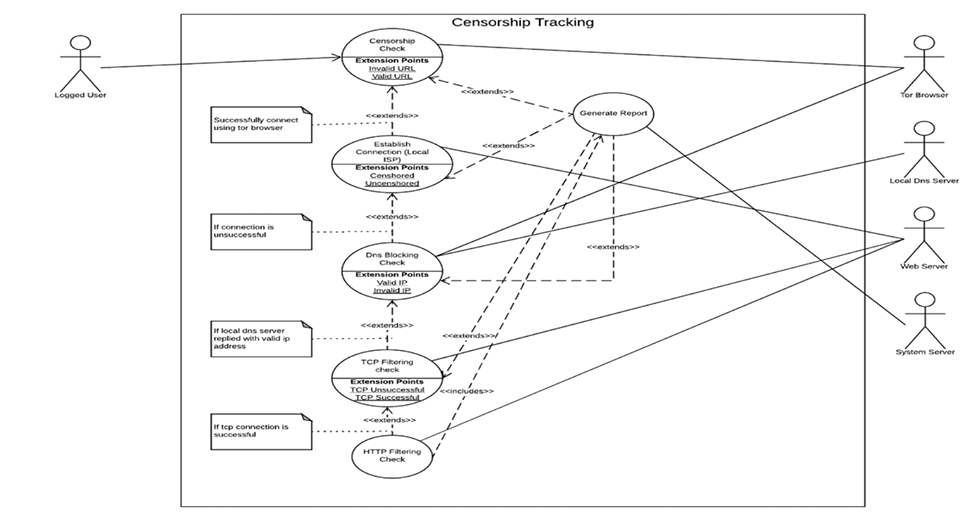
\includegraphics[width=\textwidth]{ucct.png}
    \caption{Use Case of Censorship Tracking}
    \label{fig:ucct}
\end{figure}
In this subsystem, we will implement the whole Censorship checking tests that we previously implemented independently. First we will check for DNS censorship, if we cannot conclude that DNS censorship exists, then we will check for TCP filtering censorship. Failing to conclude that, we will finally test for HTTP related censorship. The techniques used here are very much similar to the techniques used in the independent subsystems. 

%----------------- Use case General ----------------------------------
\newpage
\subsection{General Facility Use Case}

\begin{figure}[h]
    \centering
    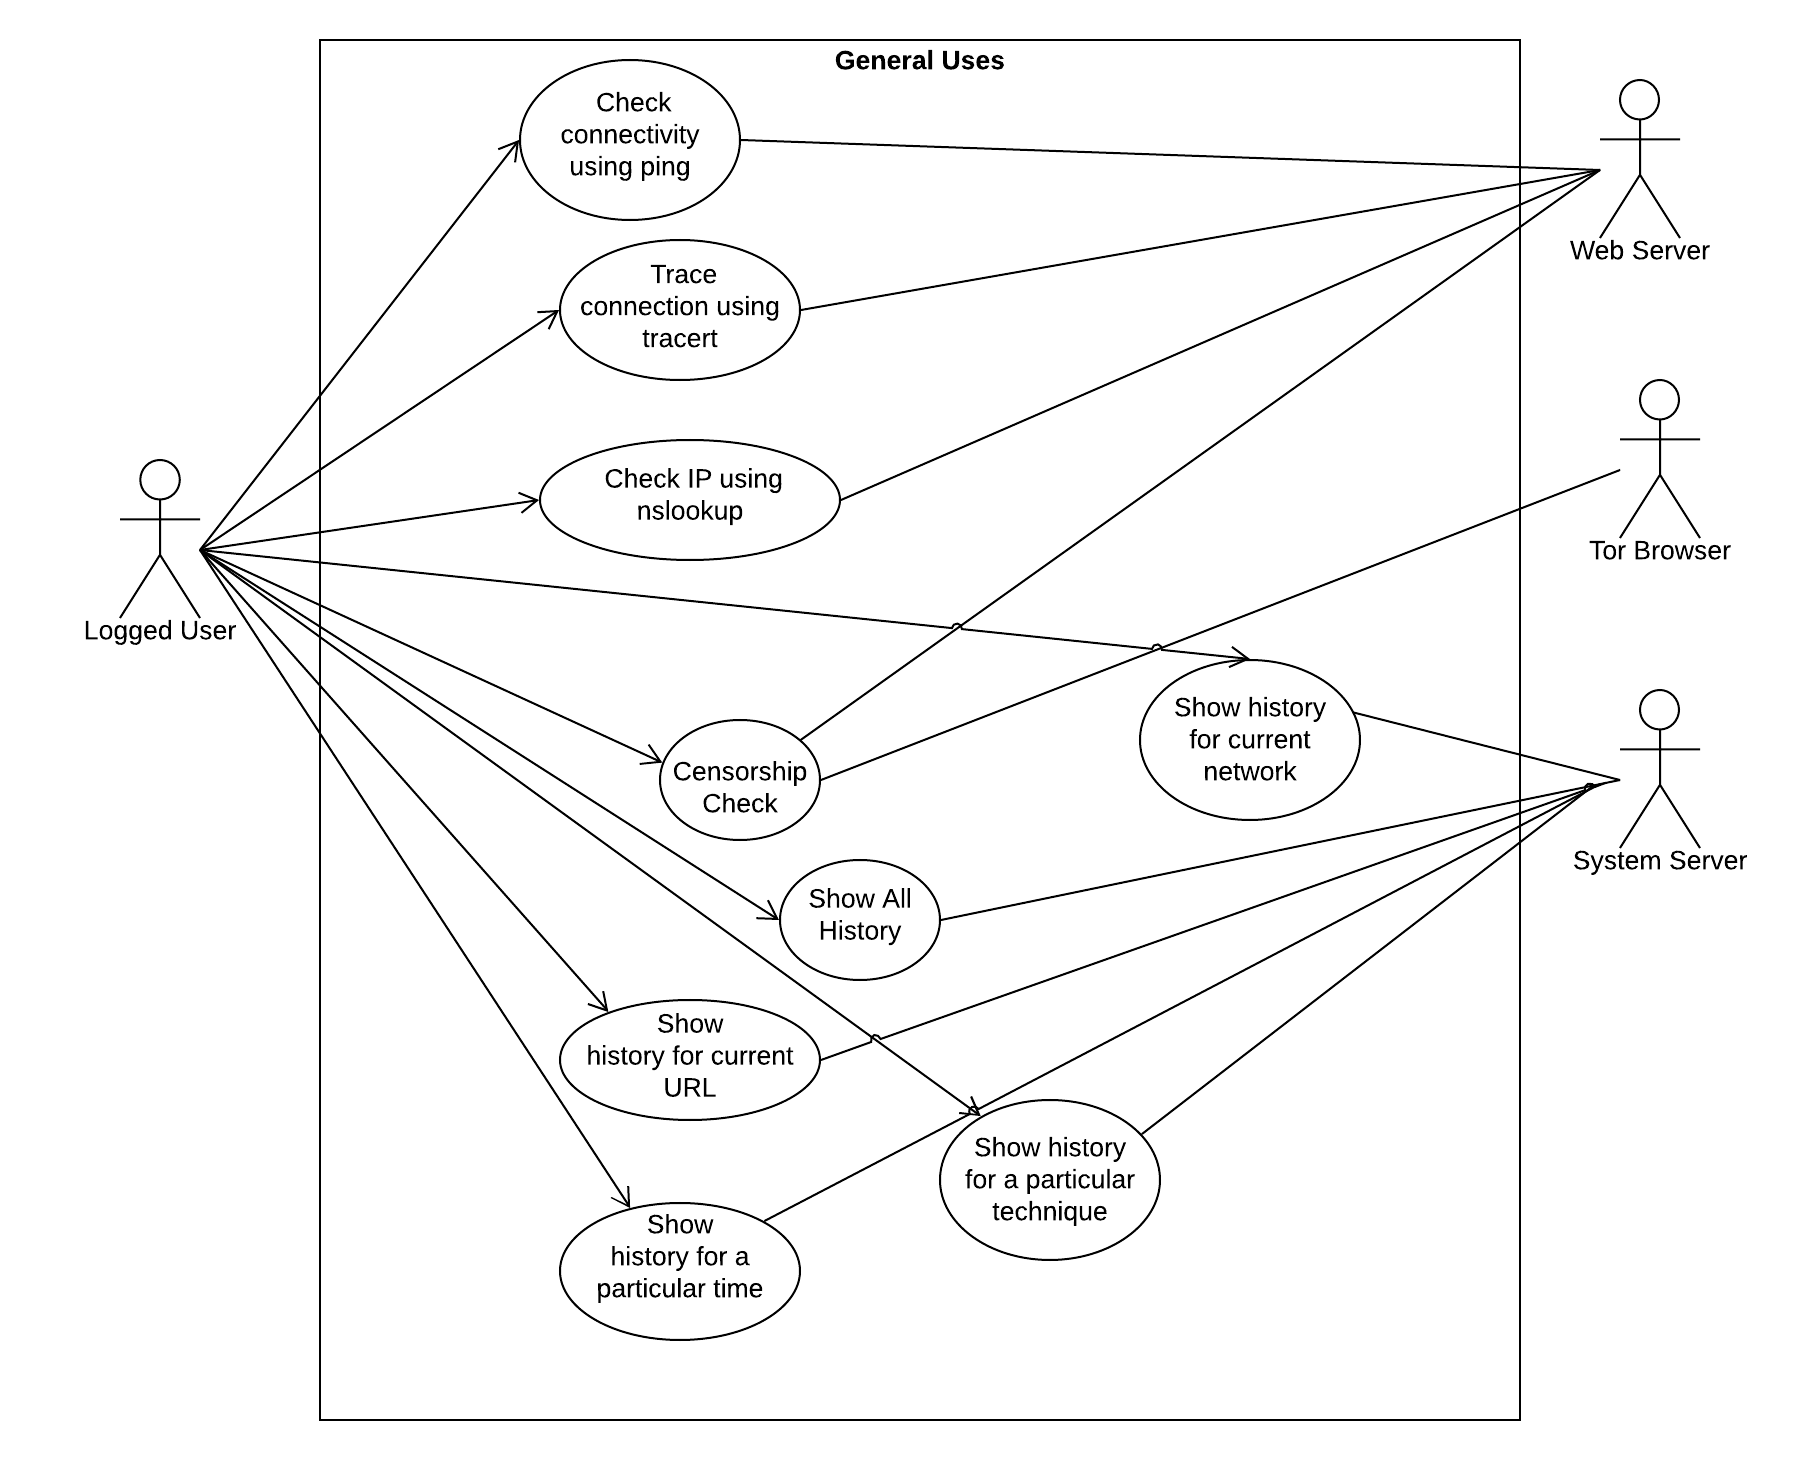
\includegraphics[width=\textwidth]{ucgc.png}
    \caption{Use Case of General Facility Subsystem}
    \label{fig:ucgc}
\end{figure}
This is for the users to view their history of the reports generated by the methods described above. Also, users may run normal tools like nslookup, tracert, ping from our system to explore themselves.

%--------------------- ERD----------------------------------
\newpage
\section{Entity Relationship Diagram}

\begin{figure}[h]
    \centering
    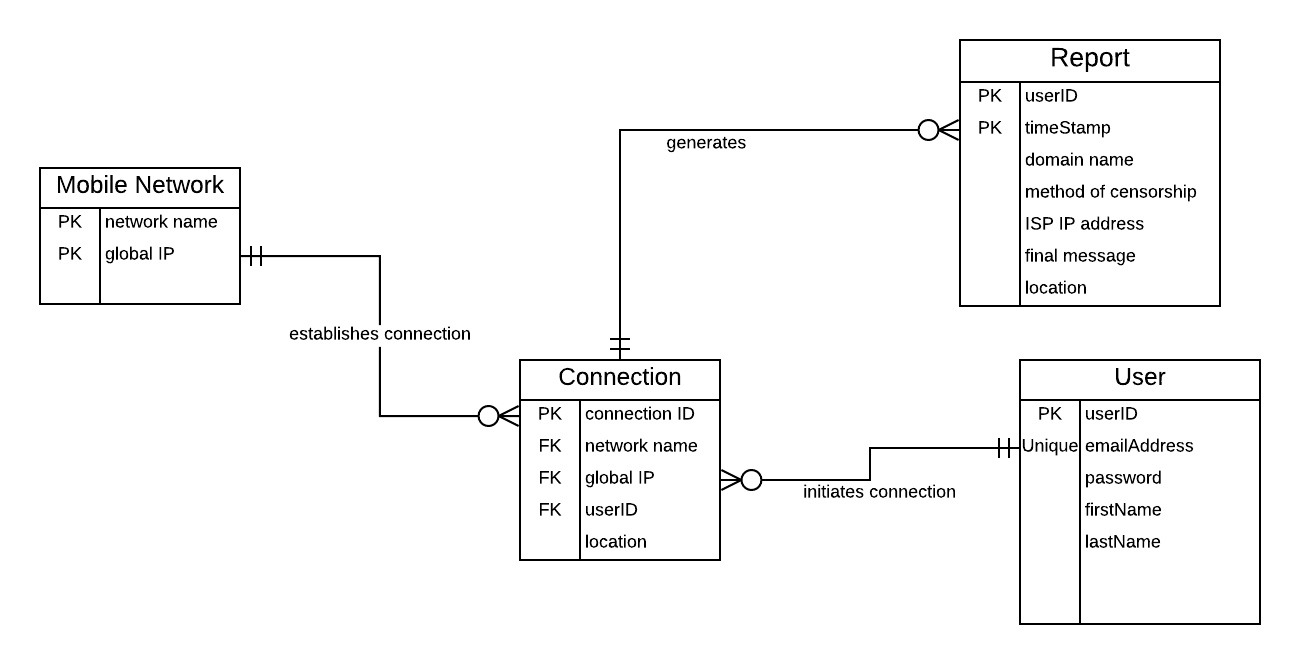
\includegraphics[width=\textwidth]{ERD.png}
    \caption{Entity Relationship Diagram for Our System}
    \label{fig:erd}
\end{figure}

%---------------Class Diagram DNS Blocking ------------------------------
\newpage
\section{Class diagrams}

\subsection{DNS Blocking Check Subsystem}
This is the class diagram of the DNS Blocking Check Subsystem.
We have followed Model-View-Controller design pattern for this subsystem.
\begin{figure}[h]
    \centering
    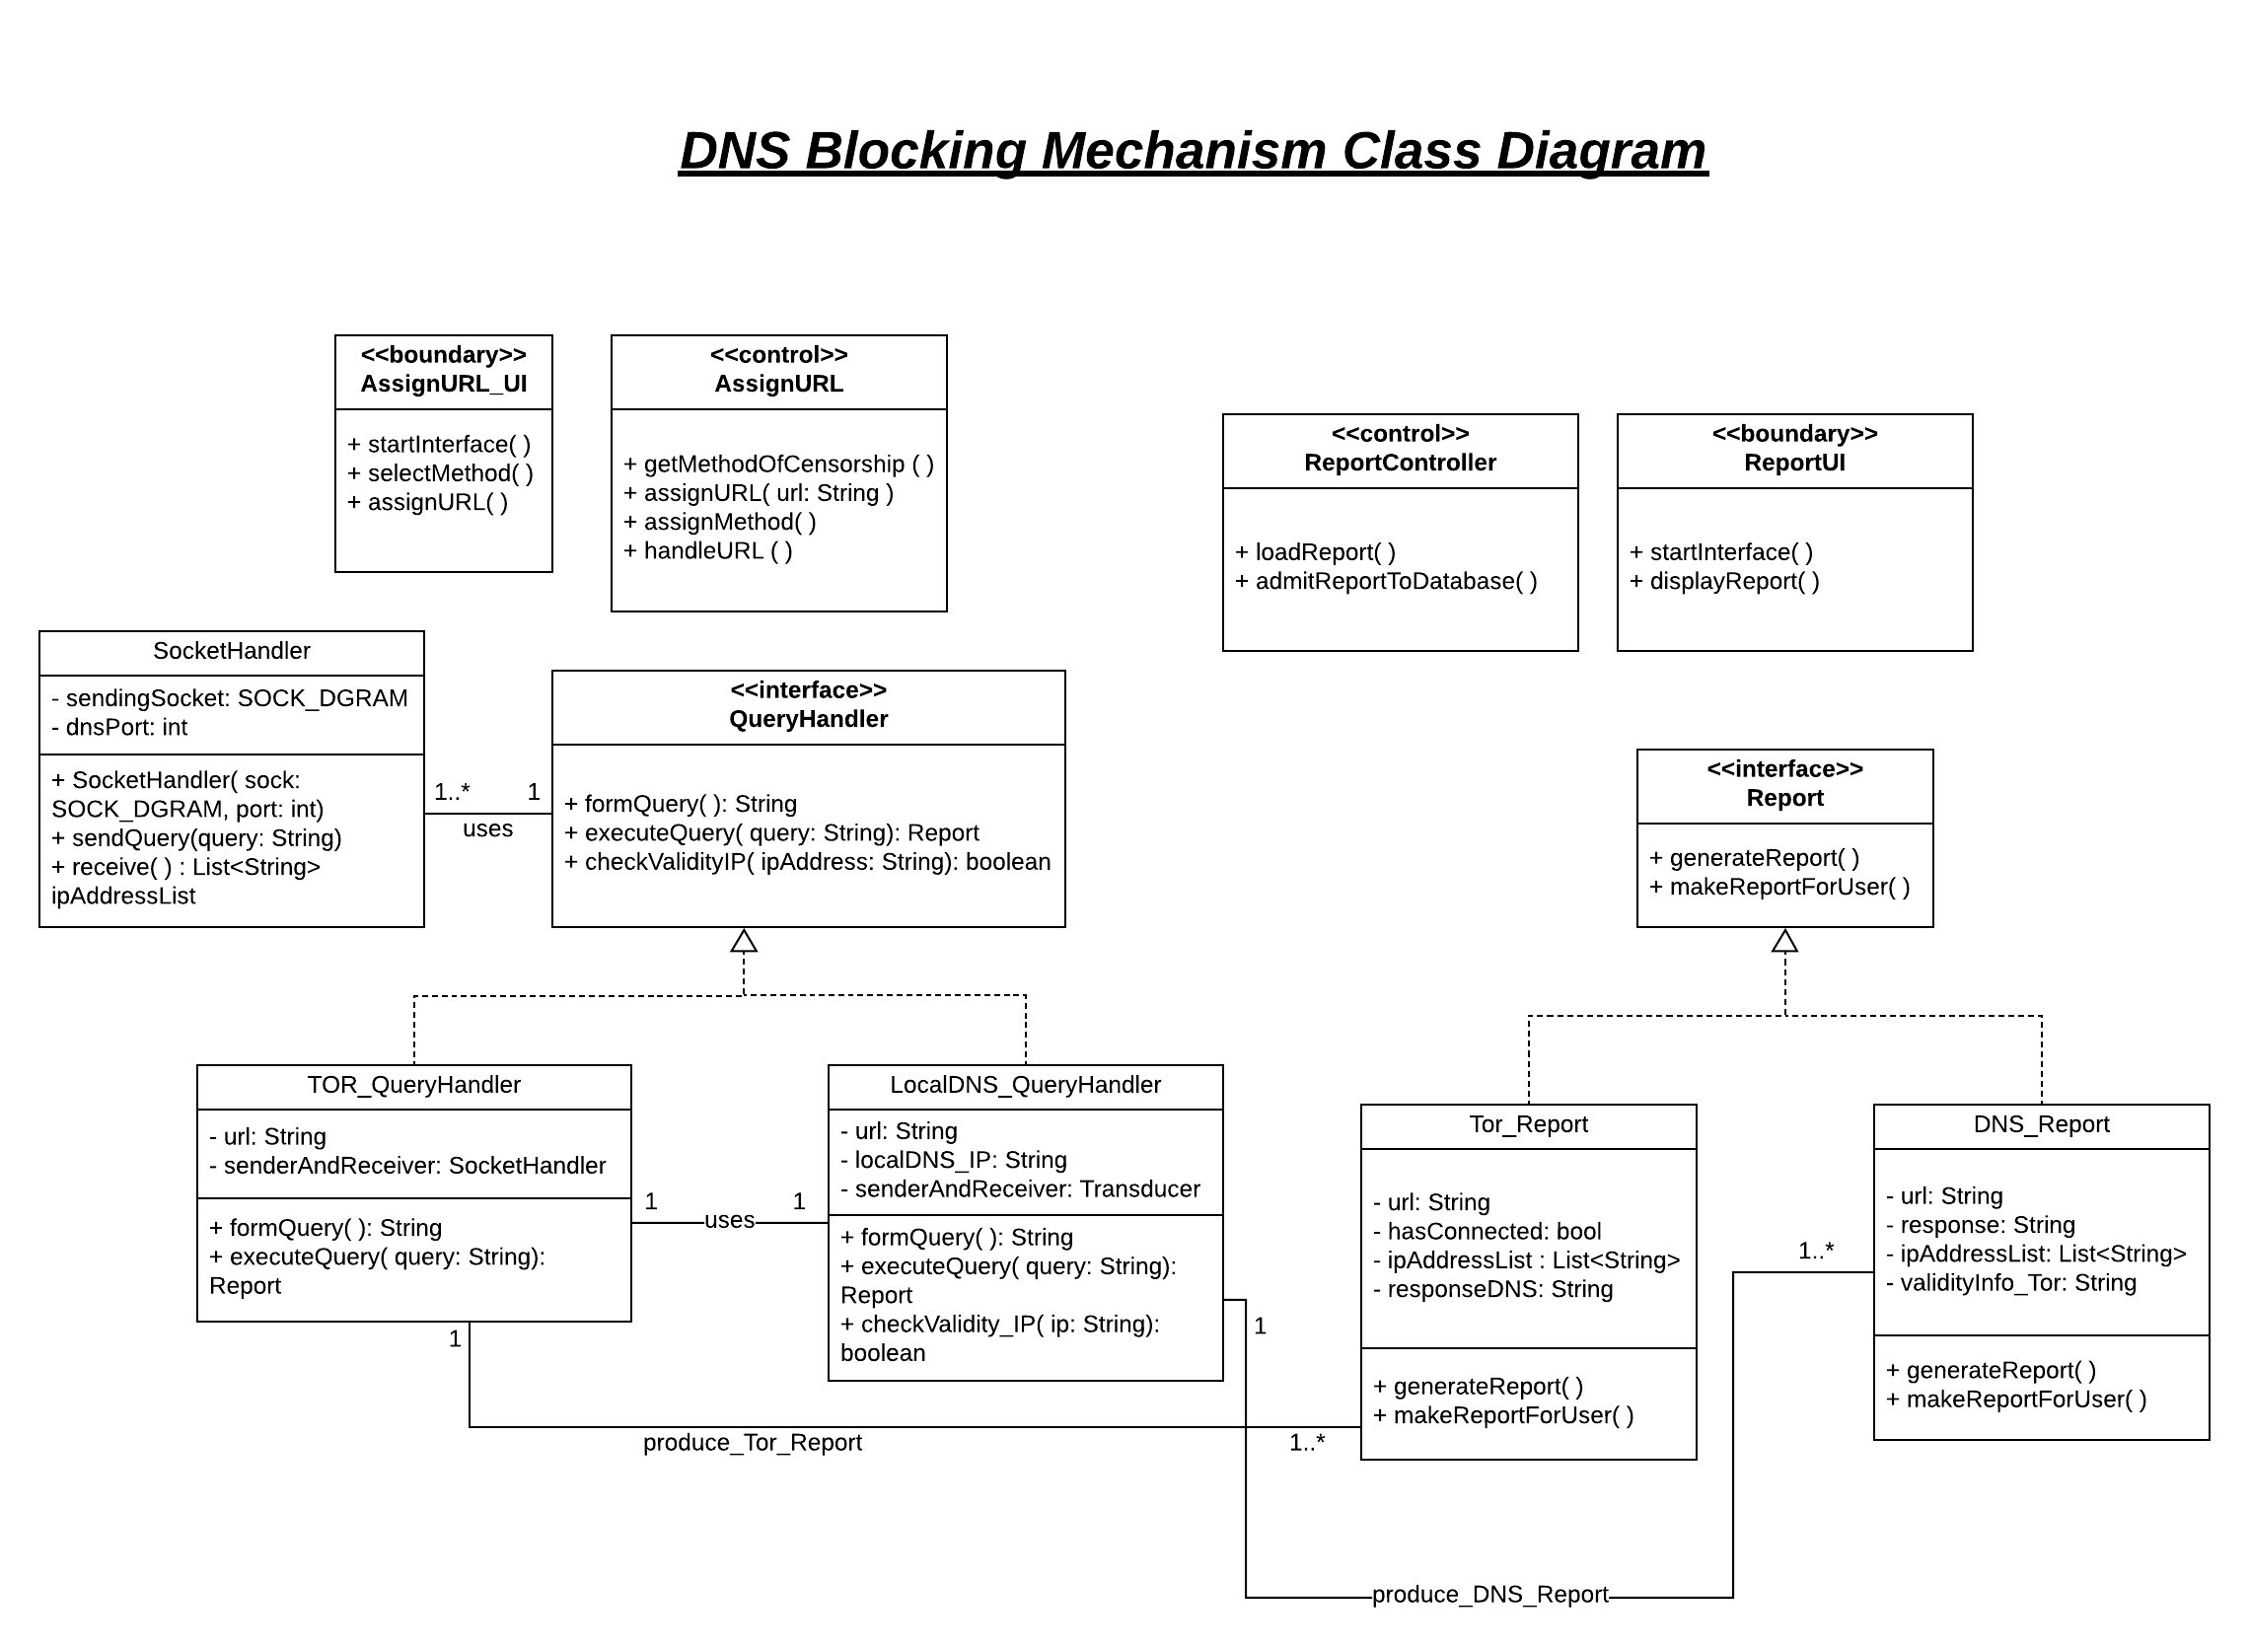
\includegraphics[width=0.8\textwidth]{cddns.png}
    \caption{Class Diagram of DNS Blocking Check Subsystem}
    \label{fig:cddns}
\end{figure}

%---------------Class Diagram HTTP Filtering ------------------------------
\newpage

\subsection{HTTP Filtering Check Subsystem}
This is the class diagram of the HTTP Filtering Check Subsystem.
We have followed Model-View-Controller design pattern for this subsystem as well.
\begin{figure}[h]
    \centering
    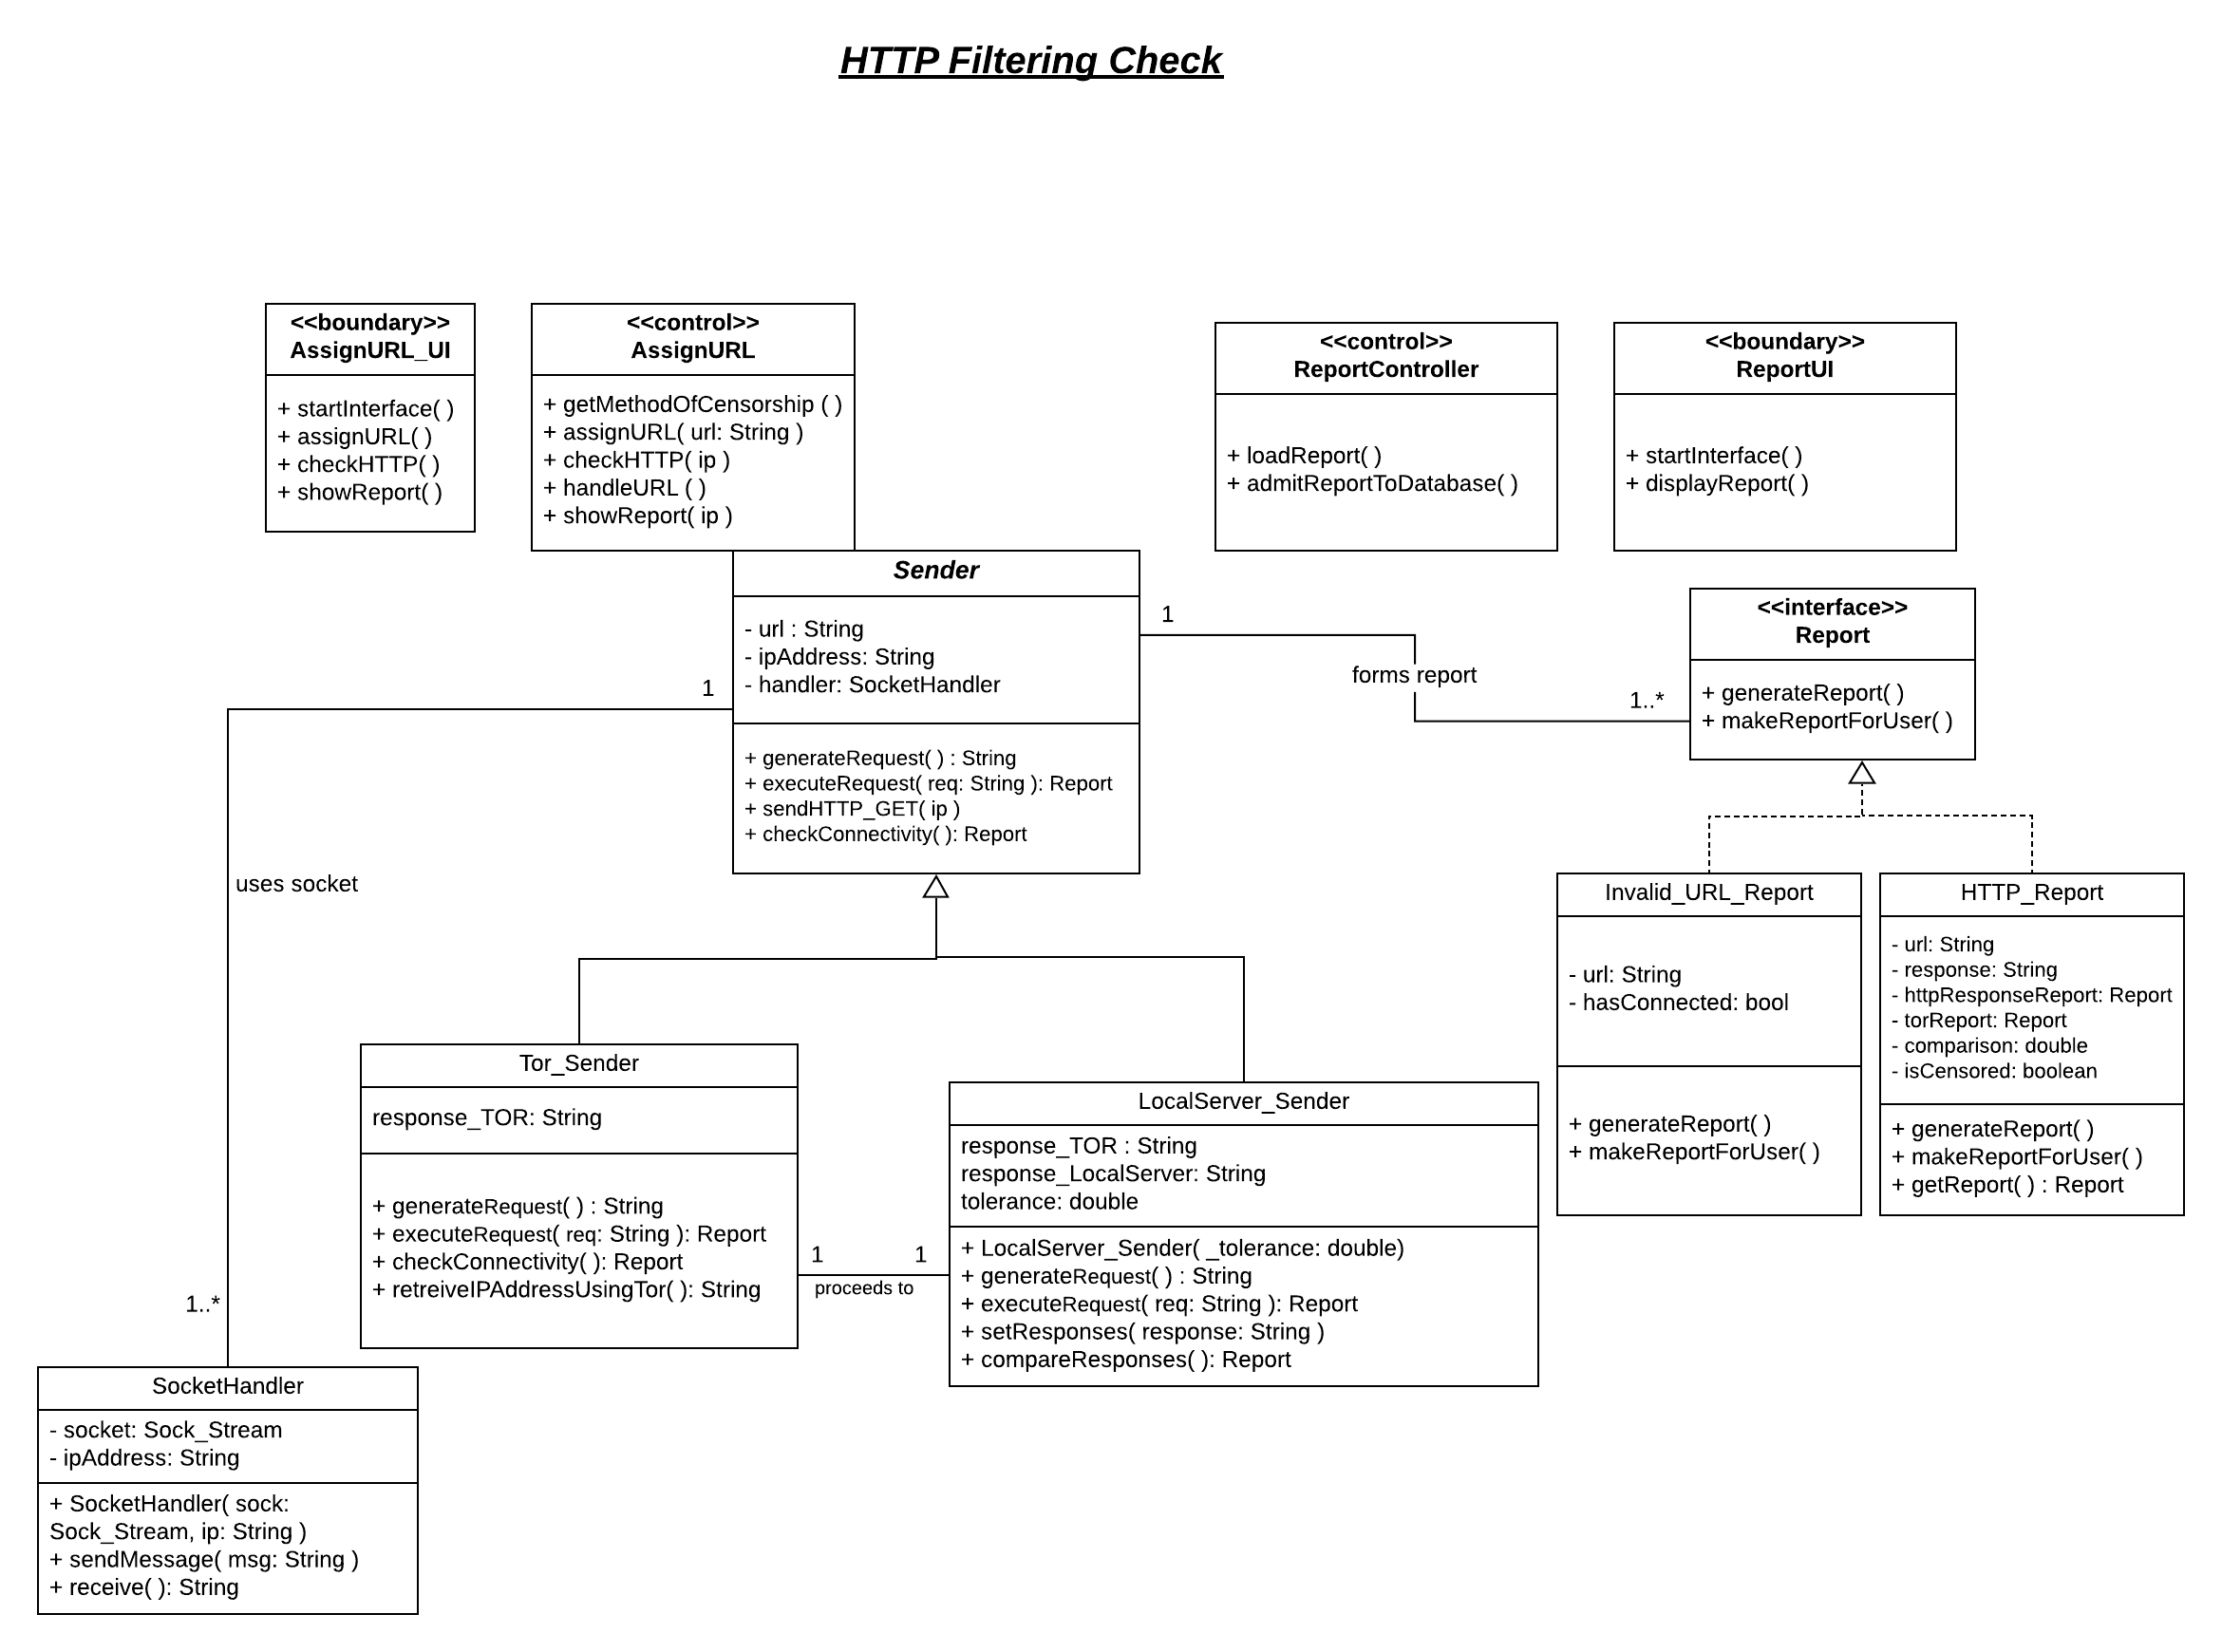
\includegraphics[width=\textwidth]{cdhttp2.png}
    \caption{Class Diagram of HTTP Filtering Check Subsystem}
    \label{fig:cdhttp}
\end{figure}

%---------------Class Diagram TCP Filtering ------------------------------
\newpage
\subsection{TCP Filtering Check Subsystem}
This is the class diagram of the TCP Filtering Check Subsystem.
We have followed Model-View-Controller design pattern for this subsystem as well.
\begin{figure}[h]
    \centering
    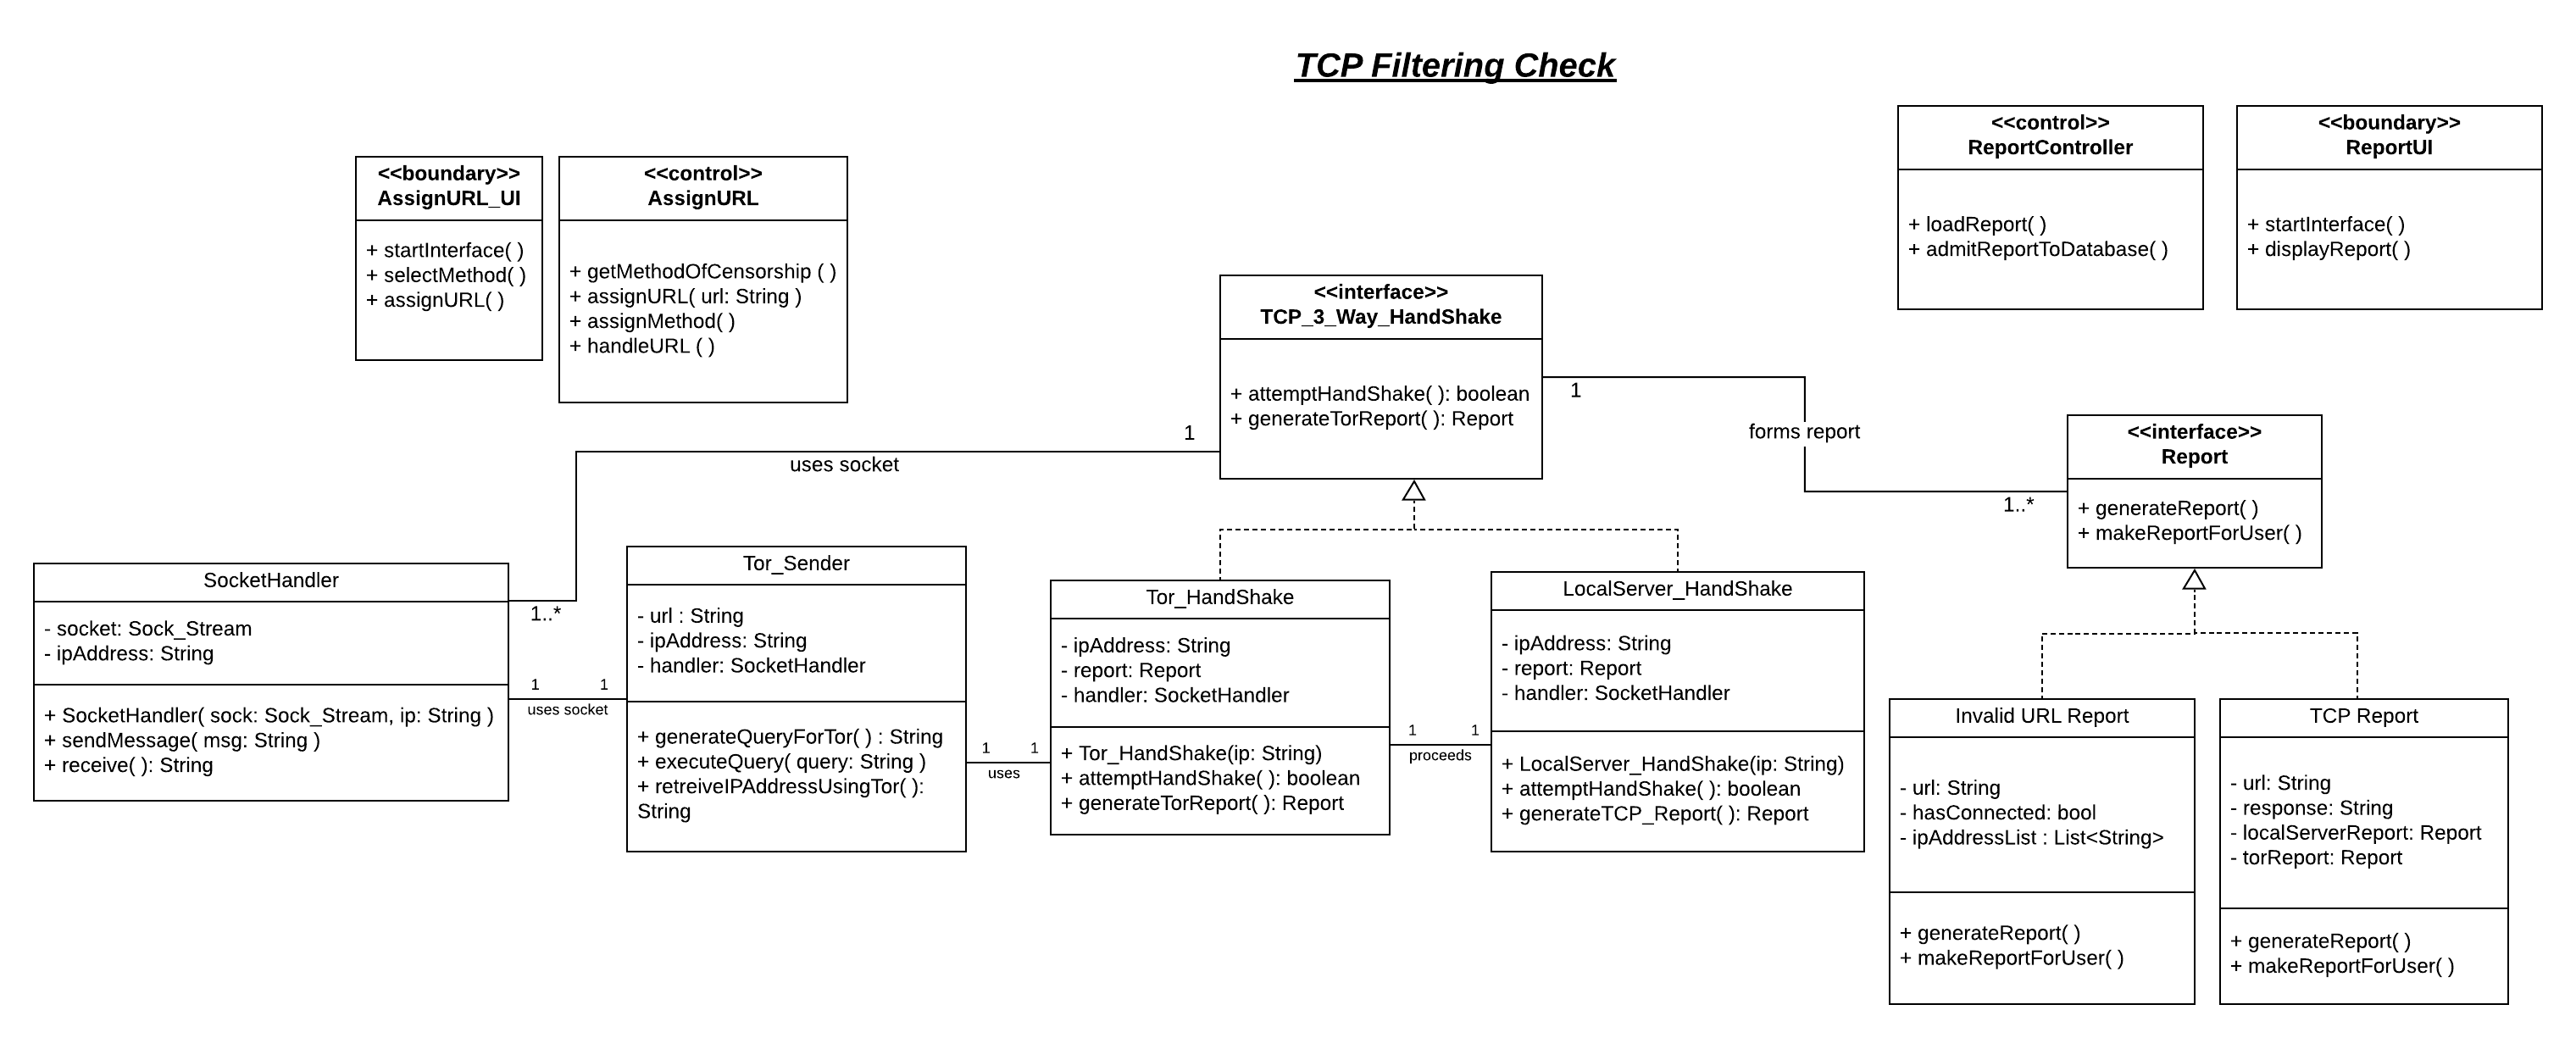
\includegraphics[width=\textwidth]{cdtcp.png}
    \caption{Class Diagram of TCP Filtering Check Subsystem}
    \label{fig:cdtcp}
\end{figure}

%----------------------- Sequence Diagrams-------------------------------------
\newpage
\section{Sequence diagram}
%----------------------- Sequence Diagram URL Validity Checker-------------------------
\subsection{URL Validity Check Sequence Diagram}
In this subsystem, first the control class starts up the initial UI window of the ui class. Then the Logged user assigns a url using assignURL() which upon receiving by the control class, it calls the getIPAddressList method using its instance of the TOR\_Sender class which instantiates a new object of Socket\_Handler class and calls the getIP\_set method. Then control is then finally returned to the user and the CheckURL\_UI class displays whether the url is valid or not to the user.
\begin{figure}[h]
    \centering
    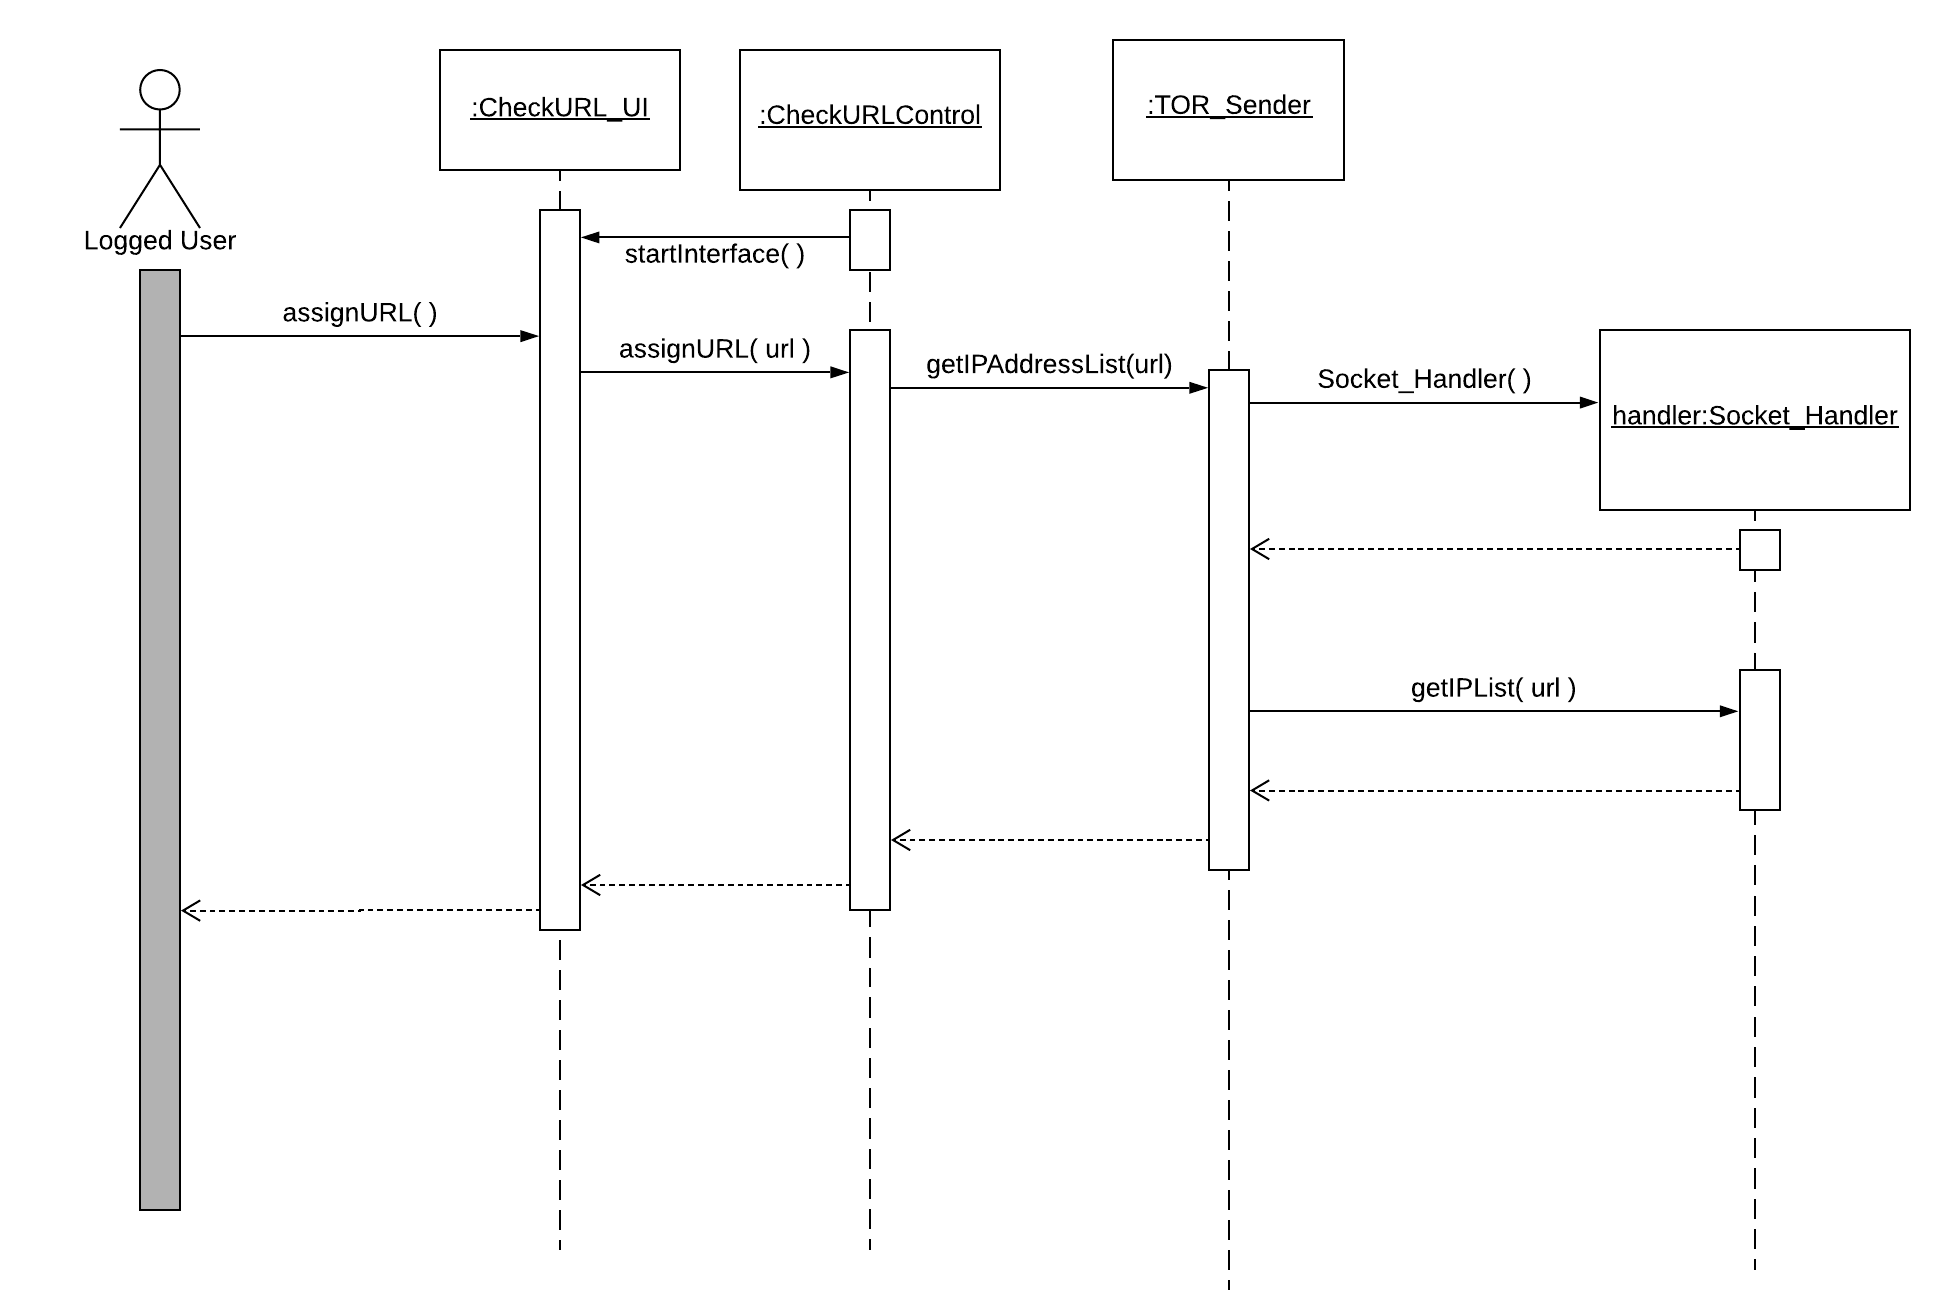
\includegraphics[width=0.8\textwidth]{seq1.png}
    \caption{Sequence Diagram of URL Validity Check Subsystem}
    \label{fig:sdvc}
\end{figure}


%----------------------- Sequence Diagram HTTP Filtering Checker-------------------------
\newpage
\subsection{HTTP Filtering Check Sequence Diagram}
In this subsystem, just like the previous one, first the control class starts up the initial UI window of the ui class. Now the logged user checks for whether HTTP filtering censorship is applied to this url. Control class calls the sendHTTP method of its instance of TOR\_Sender class. Now the instance of TOR\_Sender class instantiates a new object of Socket\_Handler class and executes HTTP GET request (and keeps the content of the request) via proxy browser (TOR Browser). Then the TOR\_Sender class's instance instantiates a new object of LocalServer\_Sender class. This does the same thing as the instance of TOR\_Sender class but now content is retrieved by sending HTTP GET request to local server (ISP) rather than proxy browser (TOR browser). Finally compareResponses method is called and a new report object is instantiated of the Report class and control is returned back to the user and the report is displayed. To further display the report again, the user may call the showReport method. 
\begin{figure}[H]
    \centering
    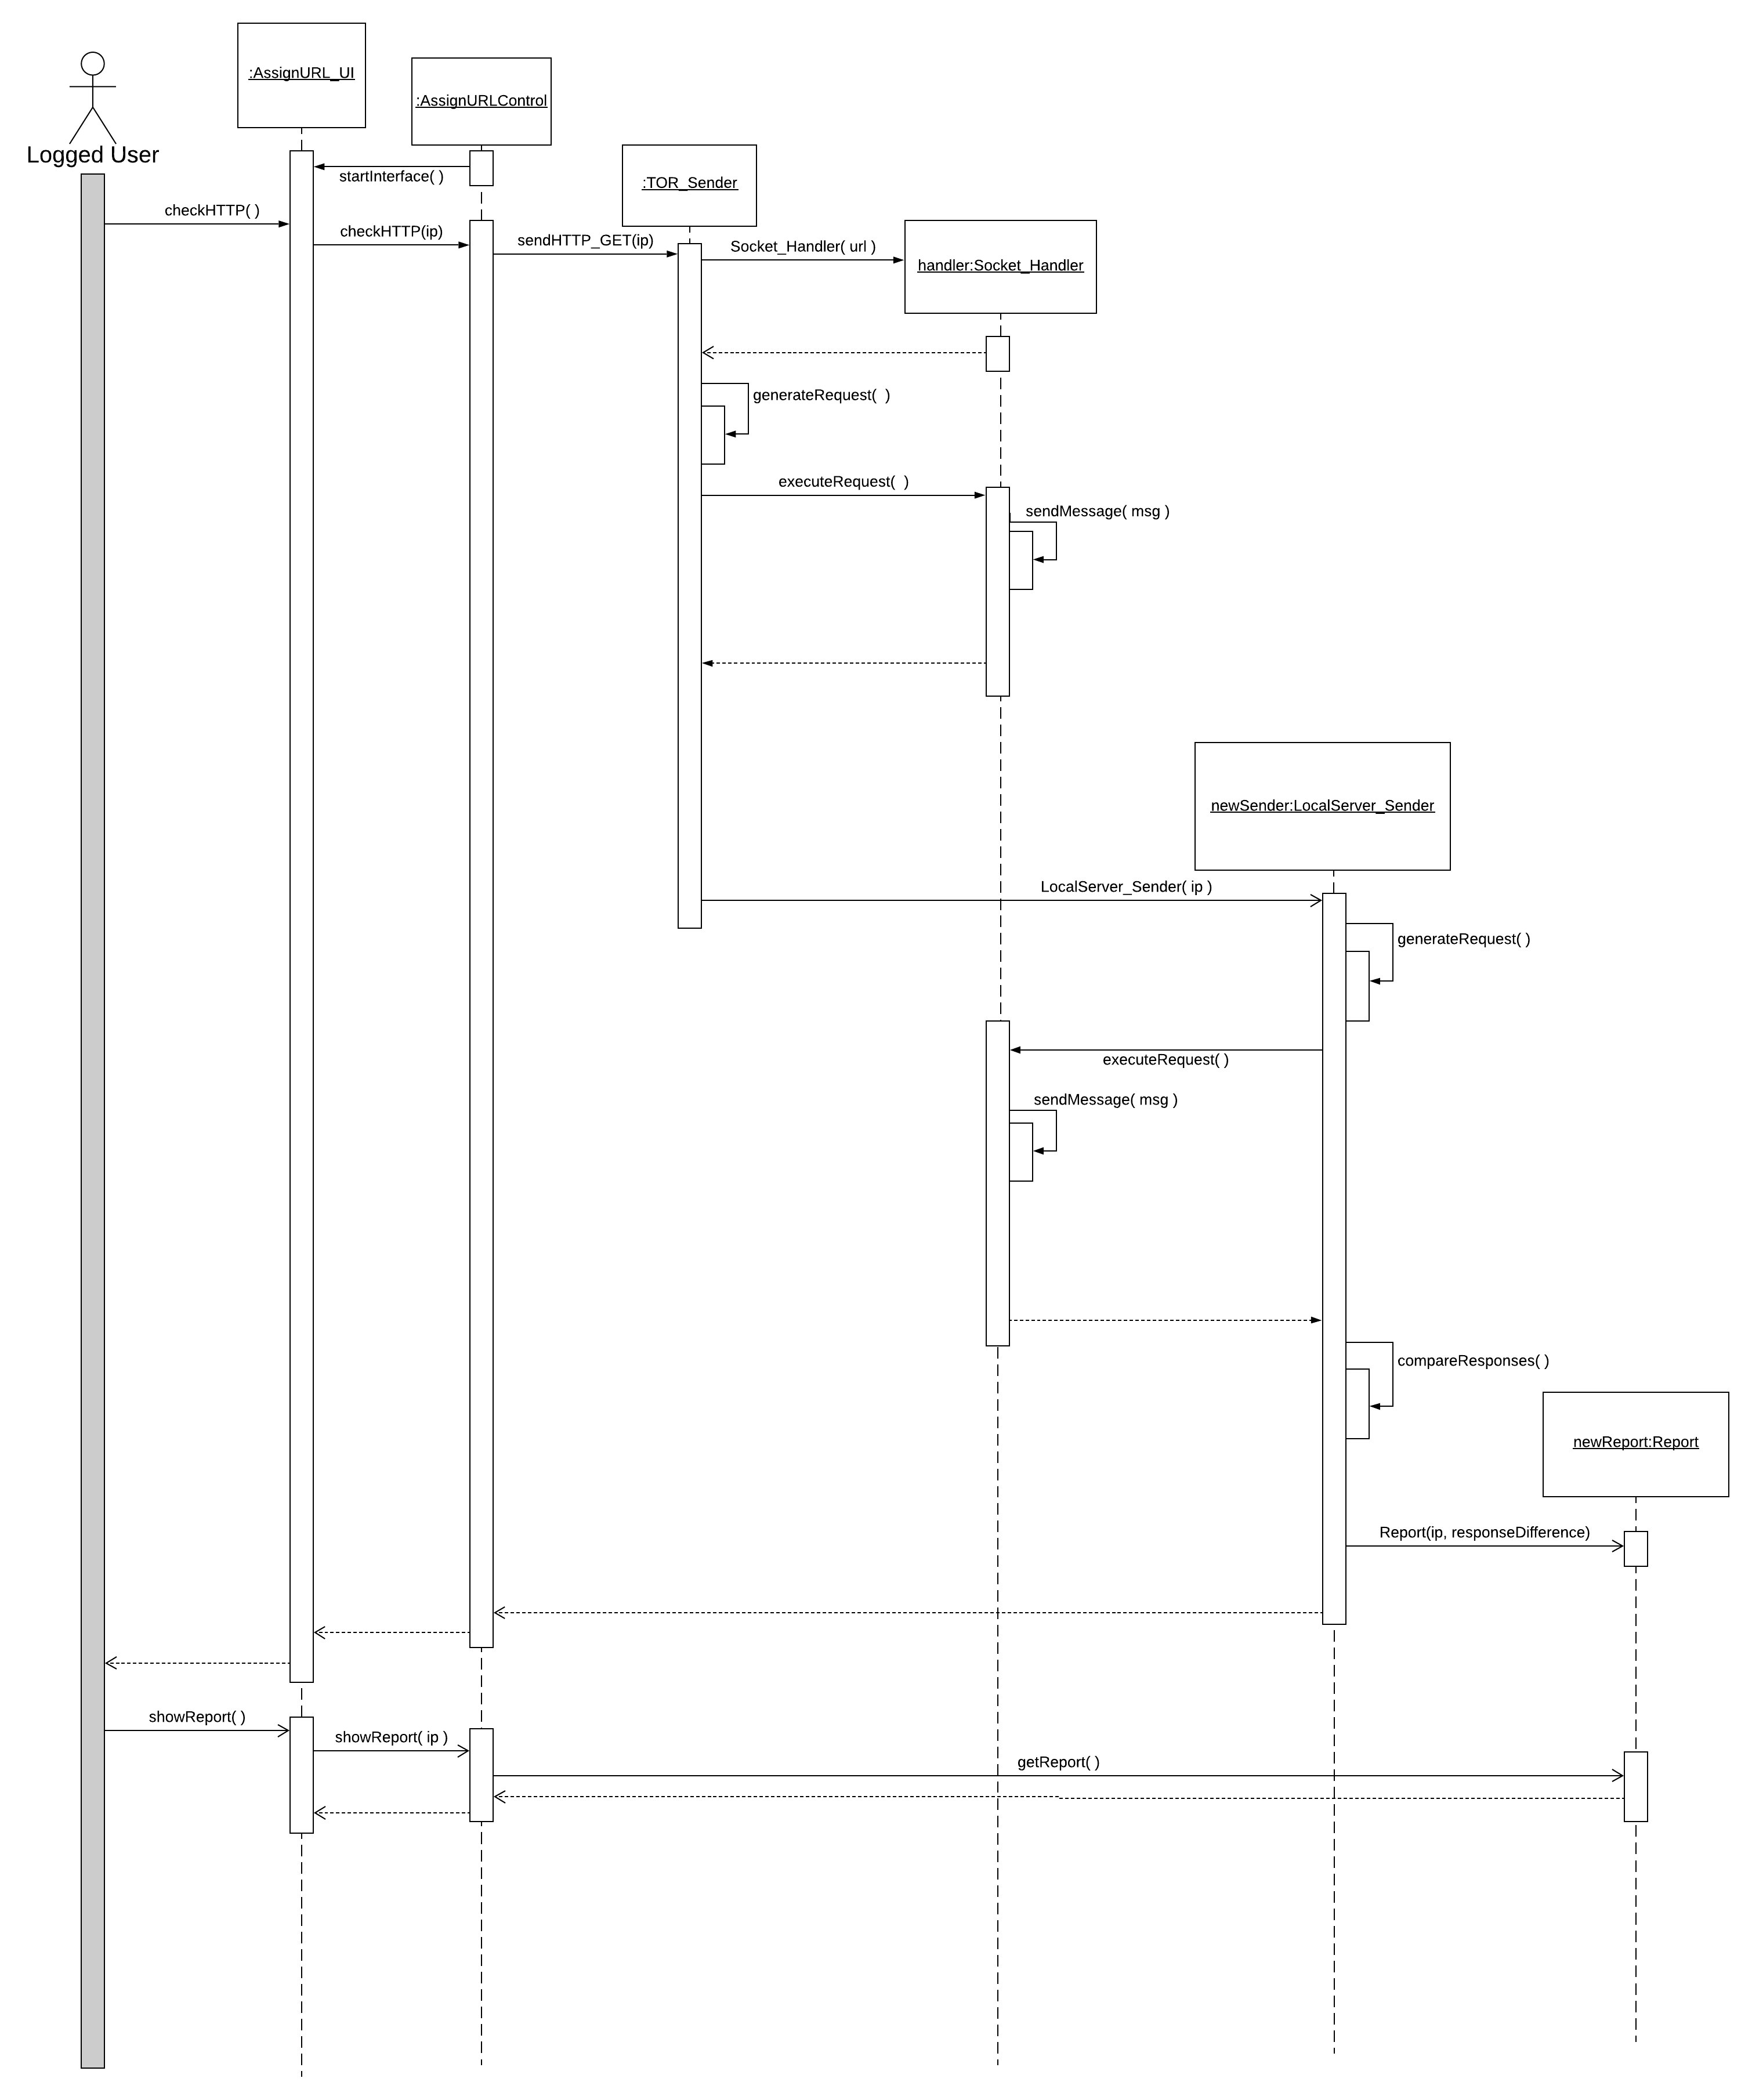
\includegraphics[width=0.84\textwidth]{seq2.png}
    \caption{Sequence Diagram of HTTP Filtering Check Subsystem}
    \label{fig:sdhttp}
\end{figure}


%----------------------- DFD  DNS Blocking Checker-------------------------
\newpage
\section{Data flow diagram}

\subsection{DNS Blocking Subsystem}


In this subsystem, Logged User (entity) sends a url to the subsystem.
Subsystem then does a dns query to Local DNS Server (Query Message), then it sends back IP address list (IP Address Set).If no IP is returned, Generate Report process is called (Null IP Report data flow) and corresponding report is stored in DNS Report Master data store.
On the other hand if IP Address set is returned, using this IP Address set, first we try to connect to TOR Browser. Depending on the response, a suitable report is generated and stored in DNS Report Master data store.

%\newpage
\begin{figure}[H]
    \centering
    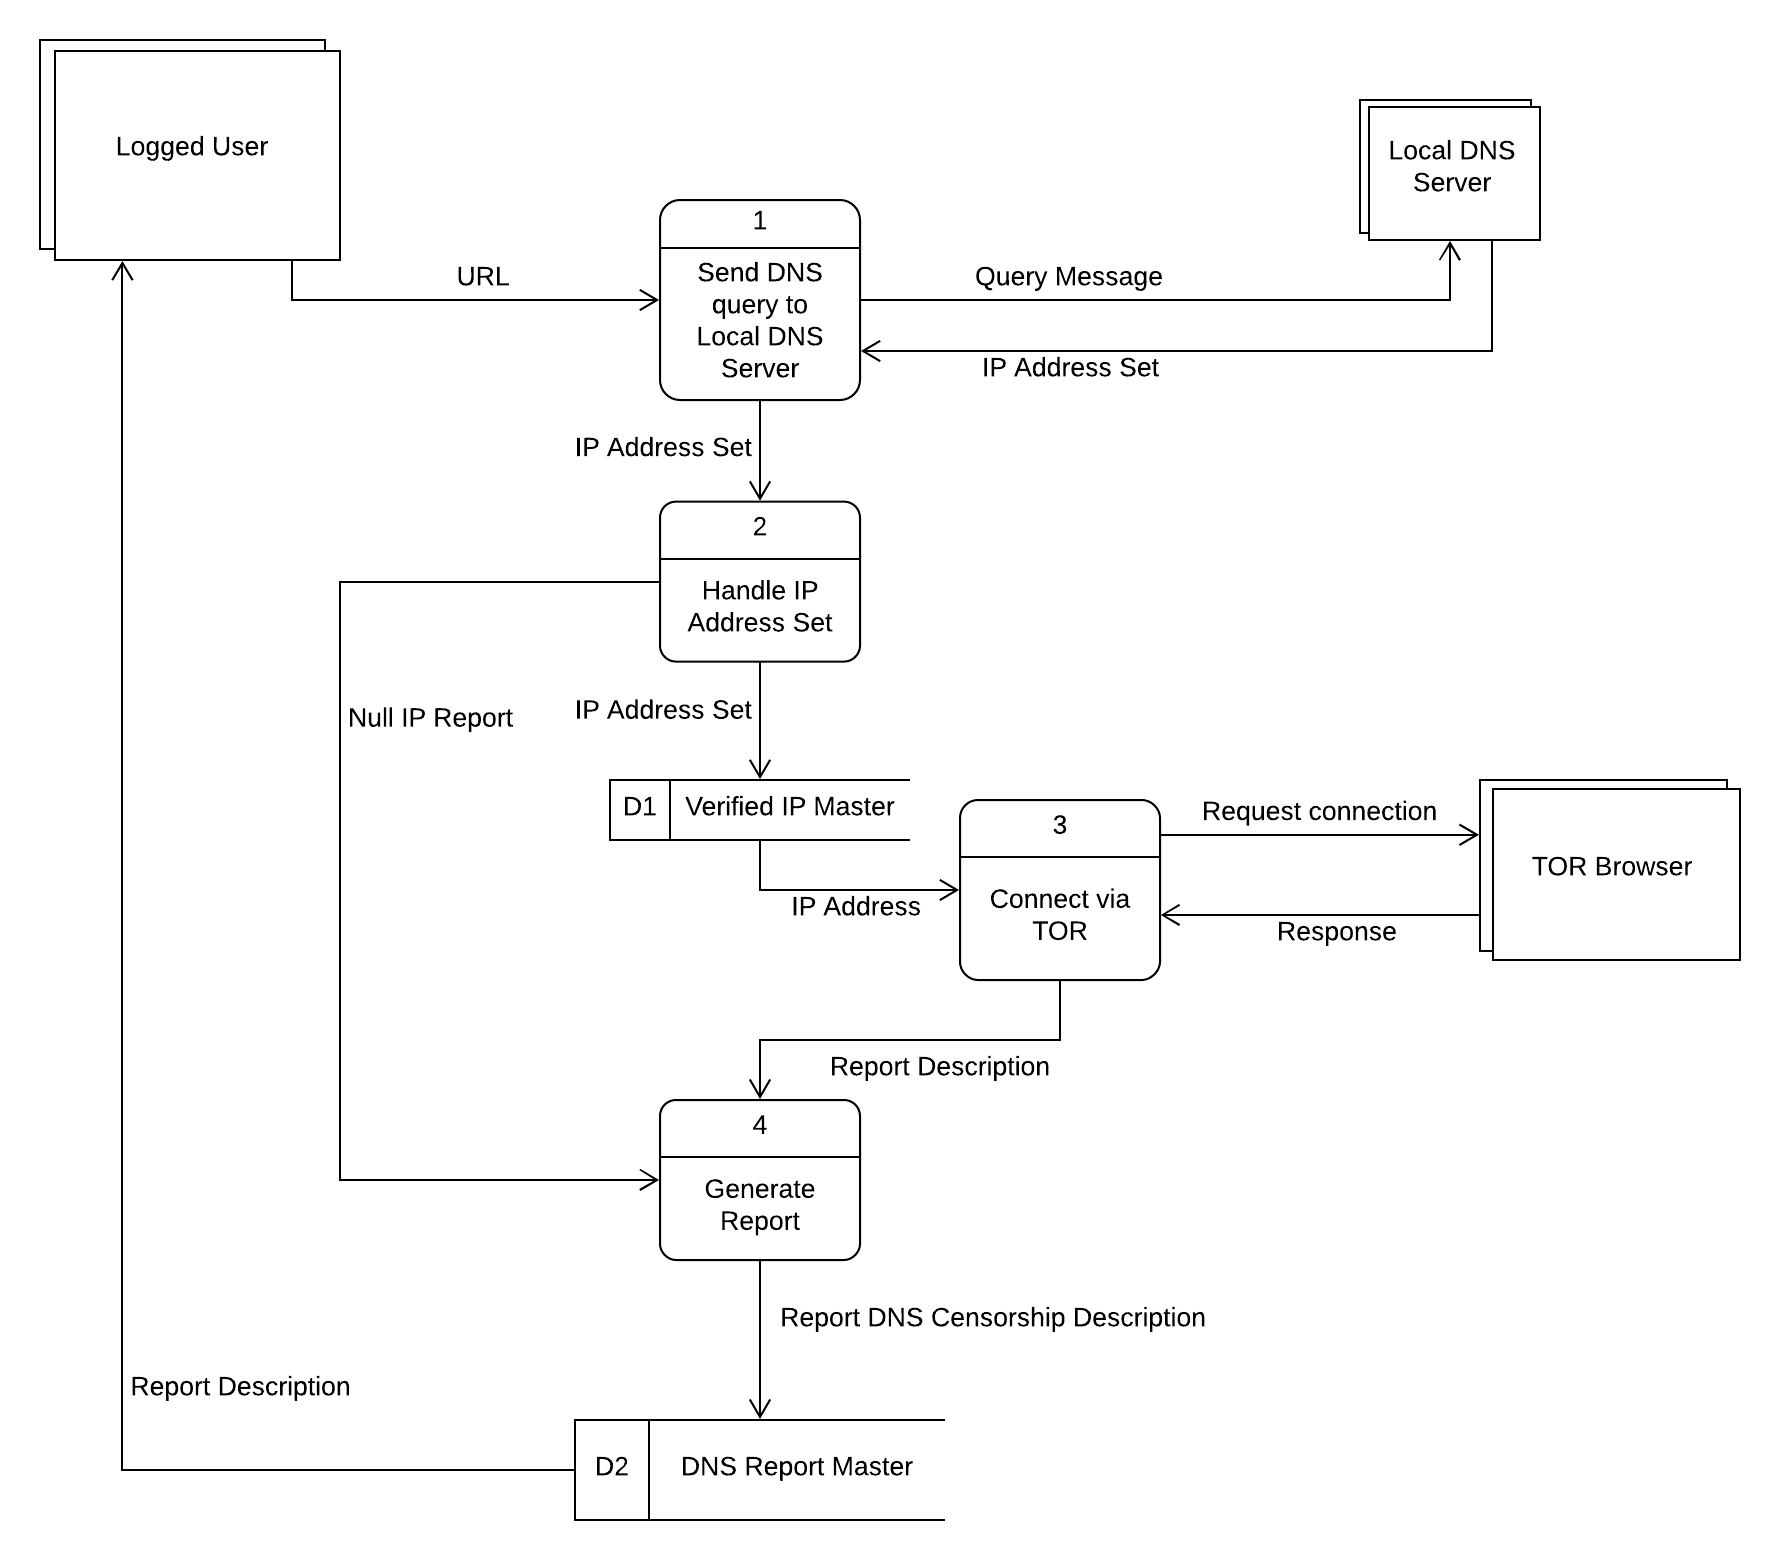
\includegraphics[width=\textwidth]{dfddns.png}
    \caption{Data Flow Diagram of DNS Blocking Subsystem}
    \label{fig:dfddns}
\end{figure}


%----------------------- DFD  TCP FILTERING Checker-------------------------

\newpage
\subsection{TCP Filtering Check Subsystem}
In this subsystem, Logged User (entity) sends a url to the subsystem.

Subsystem then sends a  query to Proxy Server, TOR Browser in this case (Query Message data flow), then it sends back IP address list (IP Address Set). Just like the previous subsystem, if no IP is returned, Generate Report process is called (Null IP Report data flow) and corresponding report is stored in DNS Report Master data store. 

On the other hand if IP Address set is returned, first it is stored in a Verified IP Master data store, then this IP Address set is used to establish TCP 3 way hand shake using proxy browser. 

If unsuccessful after multiple tries, this IP Address set is stored in IP Address Website Down Report Master data store and Generate TCP Report process is called and required report is formed and stored finally in TCP Report Master data store(D3). 

However, if proxy browser does connect, then subsystem tries to esablish TCP 3-way handshake using local server (Process 6) and generates required TCP Report using Process 5(Generate TCP Report). Final report is stored in TCP Report Master data store (D3).
\begin{figure}[H]
    \centering
    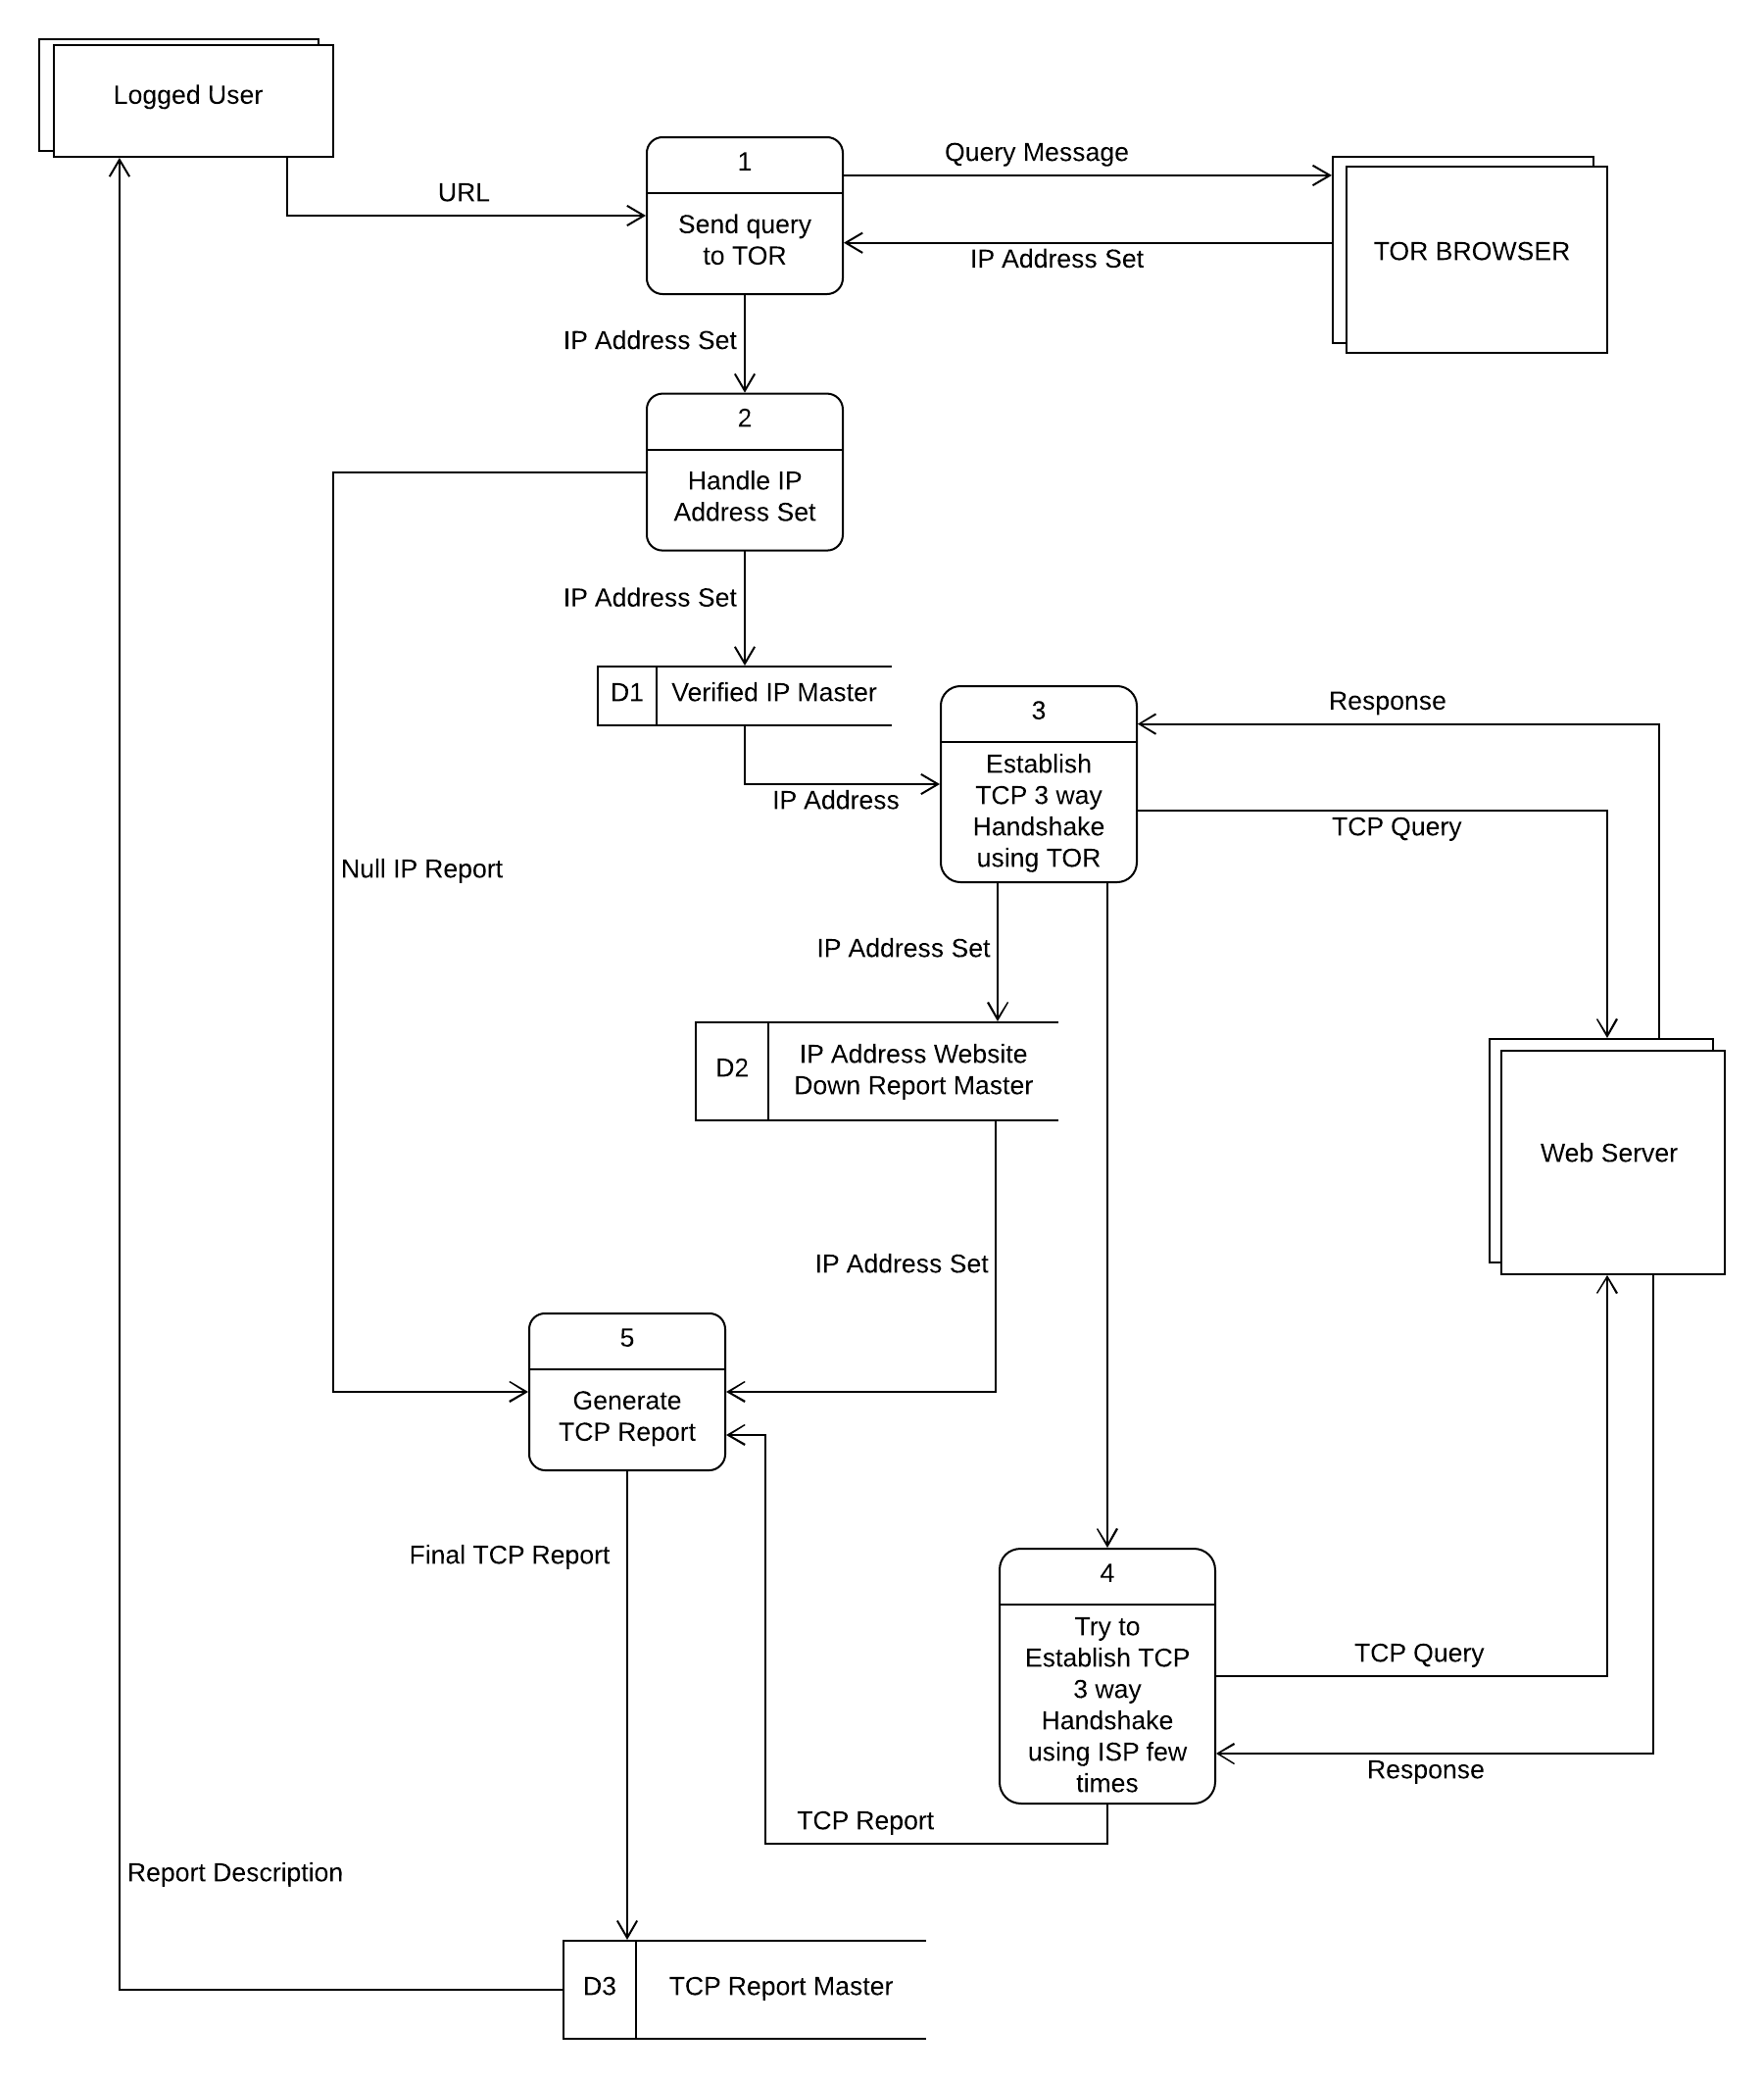
\includegraphics[width=\textwidth]{dfdtcp.png}
    \caption{Data Flow Diagram of TCP Filtering Subsystem}
    \label{fig:dfdtcp}
\end{figure}

%----------------------- Gantt Chart -------------------------
%\newpage
\section{Gantt chart}

\begin{figure}[H]
    \centering
    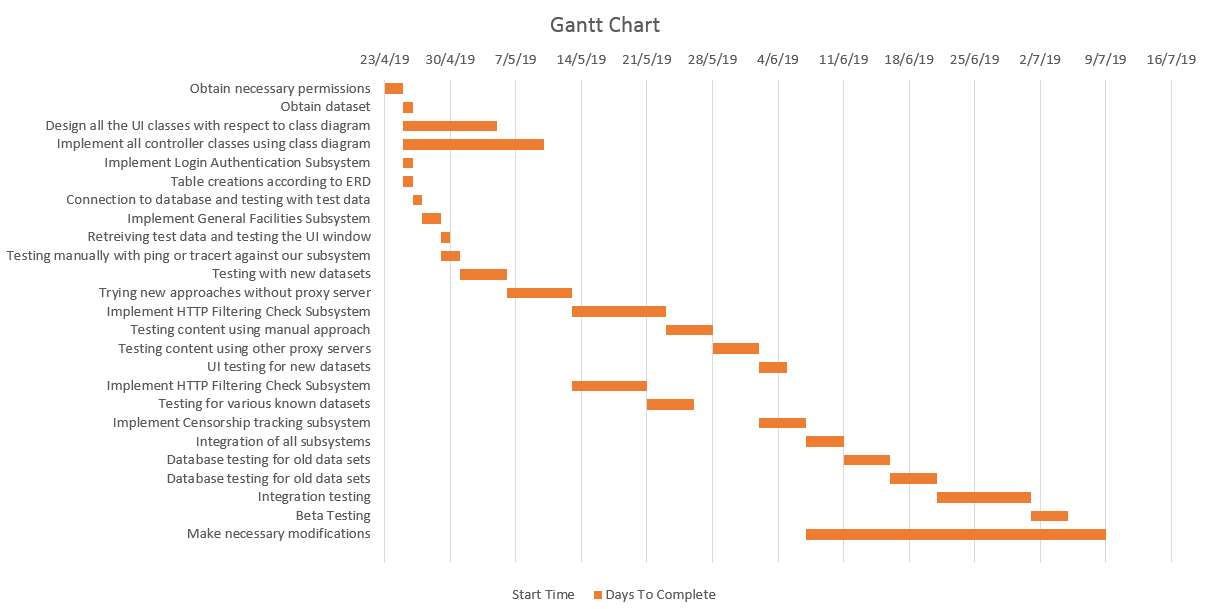
\includegraphics[width=\textwidth]{gantFinal2.PNG}
    \caption{Gantt Chart of ISP Censorship Analyzer}
    \label{fig:gantt}
\end{figure}



%----------------------- Implementation Example -------------------------
\newpage
\section{Implementation Example}

%Input UI Window
Our implementation is for the DNS Blocking Check Subsystem. Initial UI screen is simple. User may enter a single url, or by choosing a file, may enter a file where there can be multiple urls. After clicking the "Click me" button, the dns checking program runs and user can see in real time various outputs of various checkings and the final output.
\begin{figure}[H]
    \centering
    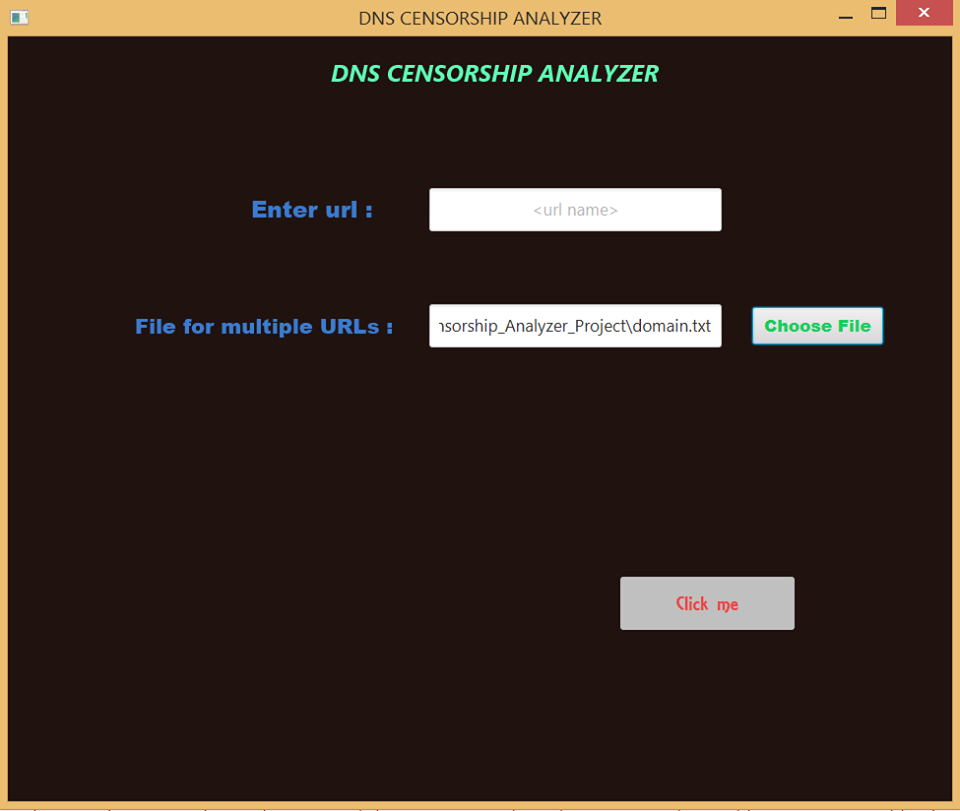
\includegraphics[width=\textwidth]{promptscreen.png}
    \caption{Input UI Window}
    \label{fig:is}
\end{figure}

\newpage

%Input file contents
\begin{figure}[H]
    %\centering
    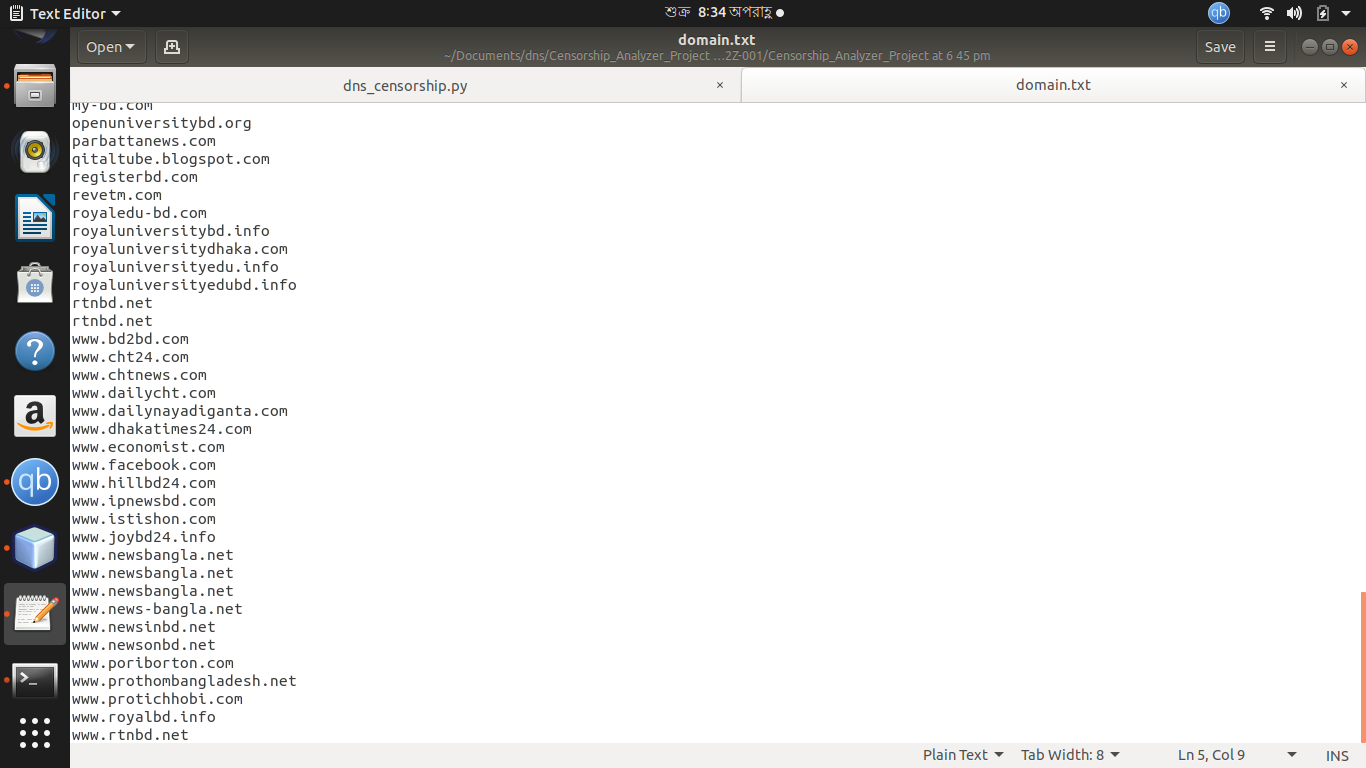
\includegraphics[width=\textwidth]{file.png}
    \caption{Sample input file}
    \label{fig:file}
\end{figure}

This is a sample input file which contains multiple urls for users to test whether dns blocking method is used for censorship or not.




%Sample output files

%Output 1 UI BOTH UNCENSORED
\newpage
\begin{figure}[H]
    \centering
    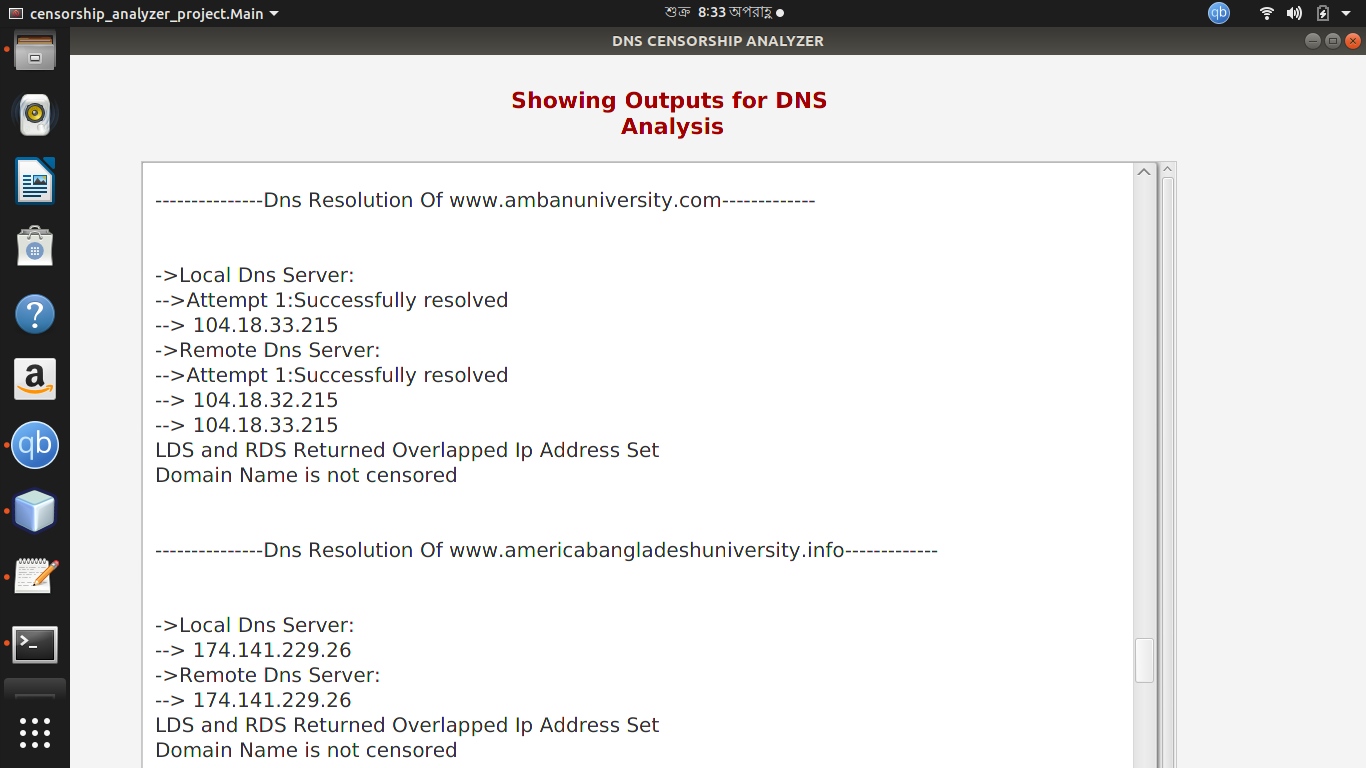
\includegraphics[width=\textwidth]{bu.png}
    \caption{DNS Censorship report (Both are uncensored)}
    \label{fig:dcr2}
\end{figure}
In this sample output of two such urls, www.ambanuniversity.com and\\ www.americabangladeshuniversity.info, we observe that Local Server(LDS) and Remote DNS Server(proxy server) has overlapping IP address set, 104.18.33.215 for www.ambanuniversity.com and 174.141.229.26 for www.americabangladeshuniversity.info, so we can conclude that DNS related censorship is not applied to either of these urls.

\newpage
\begin{figure}[H]
    \centering
    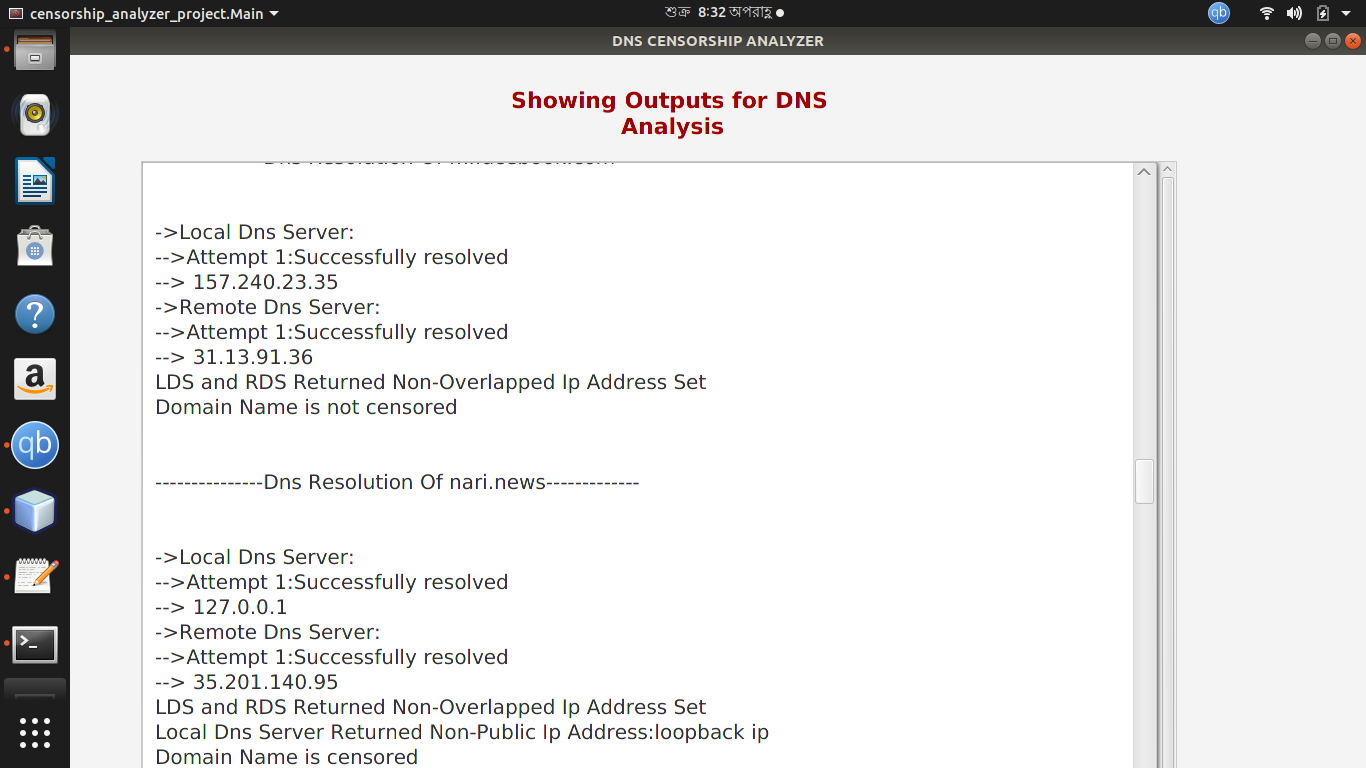
\includegraphics[width=\textwidth]{nariNews.png}
    \caption{DNS Censorship report (DNS Blocking due to Loopback IP)}
    \label{fig:dcr2}
\end{figure}
In this sample output for nari.news, local server provides a loopback ip so dns blocking can be concluded.

\newpage
\begin{figure}[H]
    \centering
    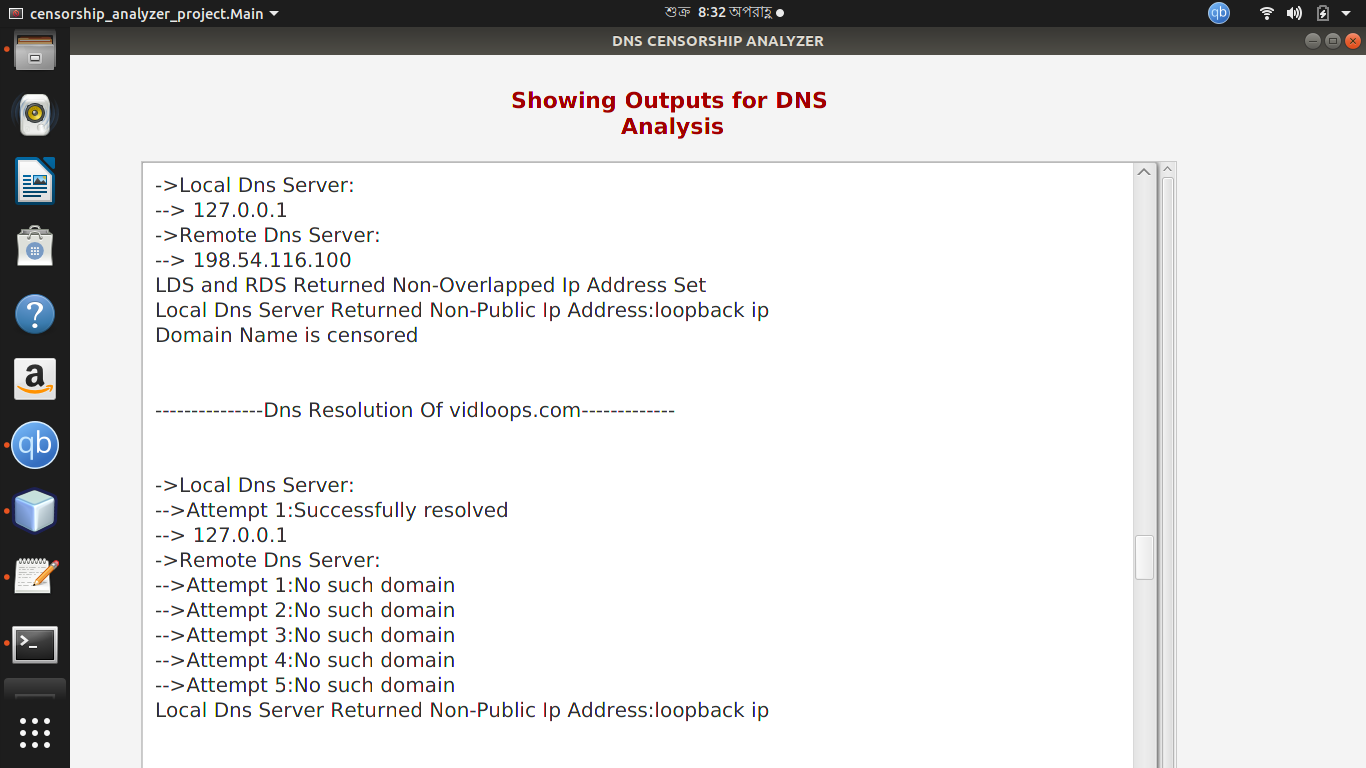
\includegraphics[width=\textwidth]{vidloops.png}
    \caption{DNS Censorship report (DNS Blocking due to Loopback IP)}
    \label{fig:dcr2}
\end{figure}
In this sample output for www.vidloops.com, local server provides a loopback ip so dns blocking can be concluded.


\newpage
\section{Conclusion}
All in all, we wish to build such a system that can detect censored websites and techniques used to censor them, with as much certainty as possible, rather than relying on existing tools such as OONI(open observatory of network interference), BlockCheck etc. We wish to add as many checking as possible for as many corner cases we can figure out. We also wish to make the system as user friendly as possible. Many benefits may come from such a system like detecting whether a url is actually censored or not when it should be. Or whether it is censored by an ISP, when it should not be. Also normal users who are eager to learn about computer networking and censorship techniques may explore this area. We hope our system may provide a starting point for such users.

\newpage
\section{References}
[1] How OONI detects HTTP Filtering? https://ooni.torproject.org/nettest/web-connectivity/.
\newline
[2] HTTP 1.1 RFC 2616. https://tools.ietf.org/html/rfc2616.
\newline
[3] Tarun Kumar Yadav, Akshat Sinha, Devashish Gosain, Piyush Sharma, Sambuddho Chakravarty.
\newline
\noindent Where The Light Gets In: Analyzing Web Censorship Mechanisms in India
\newline
https://arxiv.org/pdf/1808.01708.pdf
%\bibliography{sample}



\end{document}


